%!TEX root = ../my_thesis.tex

\renewcommand{\curChapter}{main/chapter2}

\chapter{Optimization Strategies}
\label{chap:opt}

This chapter focuses on optimization strategies dedicated to digital
communication algorithms. Our contributions are split in two parts: 1) generic
strategies and 2) specific optimizations. The two first sections describe the
generic strategies we proposed to optimize the algorithms of digital
communication receivers. Vectorization is a key of efficient software
implementations. A specific wrapper library as well as a sub-set of generic
parallelism levels are proposed. The sections afterward are dedicated to the
efficient software implementation of the algorithms for digital communication
receivers presented in the Chapter~\ref{chap:ctx}. In the last section, the
proposed contributions are summarized and discussed.

\vspace*{\fill}
\minitoccustom
\vspace*{\fill}

\newpage
\section{\MIPP: A \Cxx Wrapper for SIMD Instructions}
\label{sec:opt_mipp}

Recent articles have proposed several optimized software decoders, corresponding
to different channel codes: LDPC codes~\cite{LeGal2015,LeGal2016,LeGal2017a},
polar codes~\cite{Giard2016b,Sarkis2016,Cassagne2015c,Cassagne2016b,
Leonardon2019}, turbo codes~\cite{Zhang2012,Wu2013,Cassagne2016a,LeGal2019a}.
All of these works show the possibility to reach a good level of
\textit{computing performance} by making extensive use of SIMD (Single
Instruction Multiple Data) units. This is often achieved at the price of a
reduced \textit{flexibility}, by resorting to specific intrinsics, or by making
assumptions on the data types. However, these decoders should be implemented in
a single source code, in which the following parameters could be changed at
runtime: the channel code type, the decoding algorithm, the number of decoding
iterations, the data format, etc. Another important aspect is the
\textit{portability} of the source code on different processors (Intel\R x86,
Xeon Phi\TM KNL and ARM\R) and the possibility to use different instruction sets
(SSE, AVX, AVX-512, NEON). These three constraints (performance, flexibility,
portability) push towards the use of a SIMD library that helps in the
abstraction of the SIMD instruction sets, while still allowing a fine grain
tuning of performance.

As a foundation of the thesis work, we propose a new \Cxx SIMD library, covering
the needs in terms of expressiveness and of performance for the algorithms
dedicated to channel codes. Our contributions are:
\begin{itemize}
  \item A portable and high performance  \Cxx SIMD library called \MIPP, for
    SSE, AVX, AVX-512 and NEON instruction sets;
  \item A comparison with other state-of-the-art SIMD libraries on a Mandelbrot
    code, demonstrating that the code based on \MIPP has similar performance as
    hand-written intrinsics.
\end{itemize}
In order to let the compiler inline library calls, which is critical for the
intended SIMD programming model purpose, such library are usually header-only.
Thus, we refer to them as \textit{wrappers} instead of \textit{libraries}.
The \MIPP programming model is built on top of intrinsics, enabling a good
control on performance, but still provides an abstraction on the basic types
used in vectors (ranging from double to byte) and complex operations (parametric
reductions, log, exponential, ...).

The \longMIPP library (\MIPP) is a portable wrapper for SIMD intrinsics written
in the \Cxx language. It relies on \Cxx compile-time template specialization
techniques to replace supported generic functions with inline calls to their
intrinsics counterpart, for a given instruction set. While \MIPP is mostly
written in \Cxy{98}, it requires a \Cxy{11}-compliant compiler due to the use of
convenient features such as the \verb|auto| and \verb|using| keywords. \MIPP is
open-source (under the MIT license) and available on GitHub\footnote{\MIPP
repository: \url{https://github.com/aff3ct/MIPP}}.

\MIPP provides two application programming interface levels. The
\emph{Low Level Interface} (low) implements a basic thin abstraction layer
directly on top of the intrinsics. The \emph{medium level interface} (med.),
built on top of \MIPP low, abstracts away more details to lessen the effort from
the application programmer by relying on object encapsulation and operator
overloading.

\subsection{Low Level Interface}

\MIPP low is built around a unified \verb|mipp::reg| type that abstracts vector
registers. The vector register type represents hardware registers independently
of the data type of the vector elements. \MIPP uses the longest native vector
length available on the architecture. This design choice preserves programmer
flexibility, for instance in situations such as mixing fixed-point and
floating-point operations. \MIPP also defines a \emph{mask} register type
\verb|mipp::msk|, which either directly maps to real hardware masks on
instruction sets that support it (such as AVX-512), or to simple vector
registers otherwise.

\MIPP low defines a set of functions working with \verb|mipp::reg| and
\verb|mipp::msk|. This set is organized into eight families: memory accesses,
shuffles, bitwise boolean arithmetic, integer operations, float. operations,
mathematical functions, reductions, and mask operations.

In the AVX-512 instruction set, one \textit{regular} vector operation plus one
masking operation can be performed in a single CPU clock cycle. For instance,
the following instruction \verb|"m ? a+b : src"| performs an addition and a
masking operation:

\mint{C++}|__m512 _mm512_mask_add_ps(__m512 src, __mmask16 m, __m512 a, __m512 b);|
{\noindent
\MIPP natively supports such operations with the \verb|mipp::mask| function. The
previous example becomes in \MIPP:
}
\mint{C++}|mipp::mask<float,mipp::add<float>>(m, src, a, b);|
{\noindent
For instruction sets without masking support, the \verb|mipp::mask| call is
expanded as an operation and a blend instead.
}
\subsection{Medium Level Interface}

\begin{listing}[htp]
  \inputminted[frame=lines,linenos]{C++}{\curChapter/src/mipp/mli.cpp}
  \caption
    [\MIPP medium level interface encapsulation.]
    {Medium level interface encapsulation.}
  \label{lst:opt_mipp_mli}
\end{listing}

The \MIPP medium level interface (\MIPP med.) provides additional expressiveness
to the programmer. \verb|mipp::reg| and \verb|mipp::msk| basic types are
encapsulated in \verb|mipp::Reg<T>| and \verb|mipp::Msk<N>| objects,
respectively. The \verb|T| and \verb|N| template parameters correspond to the
type and the number of elements inside the vector register and the mask
register, respectively. In these registers, objects are typed, unlike in the
\MIPP low register basic type. This avoids to write the type when a \MIPP
function is called. The function type can then be directly selected from the
parameter type. Listing~\ref{lst:opt_mipp_mli} illustrates the template-based
encapsulation, which enables \MIPP to override common arithmetic and comparison
operators.

\MIPP med. also simplifies register loading and initialization operations. The
constructor of the \verb|mipp::Reg| object calls the \verb|mipp::load| function
automatically. Thus, a load in \MIPP low:
\mint{C++}|mipp::reg a = mipp::load<float>(aligned_ptr);|
{\noindent
can be simplified into:
}
\mint{C++}|mipp::Reg<float> a = aligned_ptr;|
{\noindent
with \MIPP med. level. An initializer list
can be used with a \MIPP med. vector register:
}
\mint{C++}|mipp::Reg<float> a = {1.f, 2.f, 3.f, 4.f};|
{\noindent
Likewise, a scalar assigned to a vector sets all elements to this value.
}

\subsection{Software Implementation Details}
\label{sec:opt_mipp_implem}

\MIPP targets SSE2, SSE3, SSSE3, SSE4.1, SSE4.2, AVX, AVX2, FMA3, KNCI, AVX-512F
and AVX-512BW instruction sets on Intel\R x86 and related architectures, as well
as NEON, NEONv2, NEON64 and NEON64v2 on ARM\R. It can easily be extended to
other instruction sets. \MIPP selects the most recent instruction set available
at compile time. For instance, a code compiled with the \verb|-march=avx| flag
of the GNU GCC compiler uses AVX instructions even if the architecture supports
SSE as well. The vector register size is determined by the instruction set and
the data type. A dedicated function returns the number of elements in a \MIPP
register:
\mint{C++}|constexpr int n = mipp::nElmtsPerRegister<T>();|
{\noindent
A shortened version of this previous function is also defined as:
\verb|mipp::N<T>()|. Whenever vectorization takes place in loops, \MIPP's
philosophy is to change the stride of the loop from one to the size of
registers. The stride can be statically determined with the \verb|mipp::N<T>()|
function. If the loop size is not a multiple of the register size, 1) a
sequential tail loop can be implemented to compute the remaining elements, 2)
the padding technique can be implemented to force the loop size to be a multiple
of the vector registers. When the instruction set cannot be determined, \MIPP
med. falls back on sequential instructions. In this case, \MIPP does not use any
intrinsic anymore. However, the compiler vectorizer still remains effective.
This mode can also be selected by the programmer with the
\verb|MIPP_NO_INTRINSICS| macro.
}

\MIPP supports the following data types: \verb|double|, \verb|float|,
\verb|int64_t|, \verb|int32_t|, \verb|int16_t| and \verb|int8_t|. It also
supplies an aligned memory allocator, that can be used with types such as the
\verb|std::vector<T,A>| vector container from the \Cxx standard library (where
\verb|T| is the vector element type and \verb|A| the allocator). The alignment
requirements are not guaranteed by the default \Cxx memory allocator. The \MIPP
memory allocator can be used as follows:
\mint{C++}|std::vector<T,mipp::allocator> aligned_data;|
{\noindent
and shortened like this: \verb|mipp::vector<T> aligned_data|.
}

\MIPP comes with a comprehensive unitary test suite to validate new instruction
set ports and new feature implementations. It has successfully been tested with
the following minimum compiler versions: \verb|g++-4.8|, \verb|clang++-3.6|,
\verb|icpc15| and \verb|msvc14.0|.

\MIPP implements a generic reduction operator based on a reduction tree, which
would be tedious to write by the application programmer, due to the sequence of
heterogeneous shuffle instructions it implies. The computational complexity of
this algorithm is $O(\log_2(N))$, with $N$ the number of elements in a register.
It can operate on \verb|mipp::reg|, \verb|mipp::Reg<T>| and
\verb|std::vector<T>|. It can also work on dynamically allocated arrays. It
provides the length of the array that is a multiple of the vector register size.
Since the function passed to the reduction operator is resolved at the compile
time, the code remains efficient. Any function with the following prototype can
be used as the reduction function:
\mint{C++}|mipp::Reg<T> func(mipp::Reg<T>, mipp::Reg<T>);|
{\noindent
E.g., the code below computes the smallest element in a register:
}
\begin{minted}{C++}
mipp::Reg<float> r = {4.f, 2.f, 1.f, 3.f};
float min = mipp::Reduction<mipp::min>::sapply(r);
\end{minted}
The \verb|min| scalar variable will be assigned \verb|1.f| as the result. For
convenience, a set of functions is predefined, based on this generic reduction
feature: \verb|hadd|, \verb|hsub|, \verb|hmul| and \verb|hdiv|.

\subsection{Related Works}

Many SIMD programming solutions to take advantage of conventional instruction
sets have been surveyed in~\cite{Pohl2016}. The existing alternatives can be
decomposed into three main models: 1)~intrinsics or assembly code; 2)~dedicated
language; 3)~dedicated library. The intrinsics or assembly approaches are
non-portable. Low-level solutions target specific architectures. They offer
maximum control to take advantage of instruction set specificities, and to fine
tune register usage. However, it is quite difficult to develop and maintain a
low-level code in the long run. Some languages have been designed to provide
programmers with SIMD programming constructs. Many of them are based on general
purpose languages extended with some kinds of annotation mechanism (e.g.
pragmas) such as OpenMP~\cite{OpenMP2013}, Cilk Plus~\cite{Robison2013} or
ispc~\cite{Pharr2012}. They offer higher expressiveness, better portability and
generally more readable code, at the expense of less programmer control, and
vectorization performance. More specialized languages, such as
OpenCL~\cite{Howes2015}, enable the programmer to retain more control, as the
counterpart of writing some more specific code. In our study, the focus is given
to the library approach since the main objectives are to maximize performance,
maximize portability and deal with existing \Cxx codes.

\subsubsection{\Cxx SIMD Wrappers}

This section and the next one propose to compare different SIMD wrappers of the
state-of-the-art. This comparison has been made in 2018 when we wrote a paper
dedicated to MIPP~\cite{Cassagne2018}. Be aware that the features of the other
wrappers presented here could have evolved since that time.

Table~\ref{tab:opt_mipp_comparison_general} and
Table~\ref{tab:opt_mipp_comparison_isa_data} compare various SIMD wrappers.
Table~\ref{tab:opt_mipp_comparison_general} is focusing on the general features
while Table~\ref{tab:opt_mipp_comparison_isa_data} is targeting the supported
instruction sets and data types. They aim to present an overview of some
prominent solutions, although they are by no means exhaustive due to the
richness of the SIMD wrapper landscape. Some of the wrappers presented, such as
\MIPP, \Vc, \BoostSIMD, \VCL and \TSIMD, have been designed in an academic
research context.

\begin{table}[htp]
  \centering
  \caption{Comparison of various SIMD wrappers: General Information and Features.}
  \label{tab:opt_mipp_comparison_general}
  \begin{tabular}{r r r r | c c c}
  \multicolumn{4}{c|}{\multirow{2}{*}{\textbf{General Information}}}      & \multicolumn{3}{c}{\multirow{2}{*}{\textbf{Features}}}\\
                &                     &                &                  &                &                    &                 \\ \hline
  \textbf{Name} & \textbf{Ref.}       & \textbf{Start} & \textbf{License} & \textbf{Math}  & \textbf{\Cxx}      & \textbf{Test}   \\
                &                     & \textbf{Year}  &                  & \textbf{Func.} & \textbf{Technique} & \textbf{Suite}  \\ \hline \hline
  \MIPP         & \cite{Cassagne2018} & 2013           & MIT              & \cmark         & Op. overload.      & \cmark          \\
  \VCL          & \cite{Fog}          & 2012           & GNU GPL          & \cmark         & Op. overload.      & \textbf{N/A}    \\
  \simdpp       & \cite{Kanapickas}   & 2013           & Boost Software   & \xmark         & Expr. templ.       & \cmark          \\
  \TSIMD        & \cite{Moller2016}   & 2016           & Open-source      & \xmark         & Op. overload.      & \textbf{N/A}    \\
  \Vc           & \cite{Kretz2012}    & 2012           & BSD-3-Clause     & \cmark         & Op. overload.      & \cmark          \\
  \xsimd        & \cite{Mabille}      & 2014           & BSD-3-Clause     & \cmark         & Op. overload.      & \textbf{N/A}    \\
  \BoostSIMD    & \cite{Esterie2012}  & 2012           & Boost Software   & \cmark         & Expr. templ.       & \cmark          \\
  \bSIMD        & \cite{Esterie2012a} & 2017           & Non-free         & \cmark         & Expr. templ.       & \cmark          \\
  \end{tabular}
\end{table}

\begin{table}[htp]
  \centering
  \caption{Comparison of various SIMD wrappers: Supported ISA and Data Type.}
  \label{tab:opt_mipp_comparison_isa_data}
  \begin{tabular}{r || c c c c c || c c | c c c c}
  {\multirow{4}{*}{\textbf{Name}}} & \multicolumn{5}{c||}{\multirow{2}{*}{\textbf{Instruction Set}}}                 & \multicolumn{6}{c}{\multirow{2}{*}{\textbf{Data Type}}}                    \\
                                   & \multicolumn{5}{c||}{}                                                          & \multicolumn{6}{c}{}                                                       \\ \cline{2-12}
                                   & \textbf{SSE} & \textbf{AVX} & \textbf{AVX512} & \textbf{NEON} & \textbf{AltiV.} & \multicolumn{2}{c|}{\textbf{Float}} & \multicolumn{4}{c}{\textbf{Integer}} \\
                                   & 128-bit      & 256-bit      & 512-bit         & 128-bit       & 128-bit         & 64      & 32                        & 64     & 32     & 16     & 8         \\ \hline \hline
  \MIPP                            & \cmark       & \cmark       & \cmark          & \cmark        & \xmark          & \cmark  & \cmark                    & \cmark & \cmark & \cmark & \cmark    \\
  \VCL                             & \cmark       & \cmark       & \cmark          & \xmark        & \xmark          & \cmark  & \cmark                    & \cmark & \cmark & \cmark & \cmark    \\
  \simdpp                          & \cmark       & \cmark       & \cmark          & \cmark        & \cmark          & \cmark  & \cmark                    & \cmark & \cmark & \cmark & \cmark    \\
  \TSIMD                           & \cmark       & \cmark       & \xmark          & \cmark        & \xmark          & \xmark  & \cmark                    & \xmark & \cmark & \cmark & \cmark    \\
  \Vc                              & \cmark       & \cmark       & \xmark          & \xmark        & \xmark          & \cmark  & \cmark                    & \cmark & \cmark & \cmark & \xmark    \\
  \xsimd                           & \cmark       & \cmark       & \xmark          & \xmark        & \xmark          & \cmark  & \cmark                    & \cmark & \cmark & \xmark & \xmark    \\
  \BoostSIMD                       & \cmark       & \xmark       & \xmark          & \xmark        & \xmark          & \cmark  & \cmark                    & \cmark & \cmark & \cmark & \cmark    \\
  \bSIMD                           & \cmark       & \cmark       & \cmark          & \cmark        & \cmark          & \cmark  & \cmark                    & \cmark & \cmark & \cmark & \cmark    \\
  \end{tabular}
\end{table}

Some others, \simdpp and \xsimd, appear to be standalone development efforts by
individual programmers or maintainers. Proprietary, closed-source solutions also
exist on the market, such as \bSIMD, which is an extended version of \BoostSIMD,
or the commercial version of \VCL. The \textit{Instruction Set} column is broken
up into five families among the most widely available on the market: NEON, SSE,
AVX, AVX-512 and AltiVec. For the sake of conciseness, we choose not to list all
the instruction sets ``sub-variants'' (such as SSE2, SSE3, etc). \simdpp et
\bSIMD propose the most comprehensive instruction set compatibility. At the
other end of the range, \xsimd and \BoostSIMD only support Intel\R SIMD
instruction sets. The \textit{Data Type} column of the table summarizes the
supported vector element types and precisions. In their public version, and at
the time of writing, \Vc does not support 8-bit integers, \xsimd does not
support 8-bit and 16-bit integers and \TSIMD does not support 64-bit data types,
to the best of our knowledge. The \textit{Features} column highlights some
additional characteristics. The \textit{Math Func.} column indicates which
wrapper supports additional mathematical sub-routines, not necessarily available
as native CPU instructions (exponential, logarithm, trigonometric functions for
instance). These sub-routines are required by algorithms such as the Box-Muller
Transform (see Section~\ref{sec:opt_simu_awgn}). The \textit{\Cxx Technique}
column indicates whether the wrapper is designed as an expression template
framework, or whether it relies on operator overloading techniques. The
expression template feature is a powerful technique to automatically drive the
rewriting of whole arithmetic expressions into SIMD hardware instructions or
instruction sequences. For instance if the user writes \verb|d = a * b + c|, the
wrapper can automatically match a \emph{fused multiply and add} instruction
(FMA). \BoostSIMD and \bSIMD extensively take advantage of this
technique~\cite{Esterie2012, Esterie2012a}. The drawbacks are that the source
code complexity of the wrapper dramatically increases. \BoostSIMD and \bSIMD
have a dependency on the Boost framework to build, and currently available \Cxx
compilers produce huge amounts of arcane error messages at the slightest mistake
in the end user program. For these reasons, we decided not to base \MIPP on the
expression template technique. As mentioned in
Section~\ref{sec:opt_mipp_implem}, maintaining SIMD wrappers, and porting them
to new instruction sets is error prone by nature, due to the large number of
routines, cryptic intrinsics names, and specific instruction set details. A
comprehensive testing suite is therefore critical to validate new development,
optimizations and ports on new instruction sets. This is why \MIPP, as well as
\Vc, \BoostSIMD, \simdpp and \bSIMD come with their own test suites. We have not
found similar test suites in the software distributions of \VCL, \xsimd and
\TSIMD. However, test suites might be in use internally, within the development
teams of these wrappers.

\subsubsection{Experimentation Platforms}
\label{sec:opt_mipp_protocol}

\begin{table}[htp]
  \tabcolsep=6pt
  \centering
  \caption
    [Specifications of the target processors for the \MIPP experiments.]
    {Specifications of the target processors.}
  \label{tab:opt_mipp_specs}
  \begin{tabular}{c | c c c c}
  \textbf{Name}                   & \textbf{Exynos5422} & \textbf{RK3399} & \textbf{Core\TM i5-5300U}  & \textbf{Xeon Phi\TM 7230} \\ \hline \hline
  \textbf{Year}                   & 2014                & 2016            & 2015                       & 2016                      \\
  \textbf{Vendor}                 & Samsung\R           & Rockchip\R      & Intel\R                    & Intel\R                   \\
  \multirow{2}{*}{\textbf{Arch.}} & ARMv7               & ARMv8           & \multirow{2}{*}{Broadwell} & Knights                   \\
                                  & Cortex-A15          & Cortex-A72      &                            & Landing                   \\
  \textbf{Cores/Freq.}            & 4/2.0 GHz           & 2/1.6 GHz       & 2/2.3 GHz                  & 64/1.3 GHz                \\
  \textbf{LLC}                    & 2 MB L2             & 1 MB L2         & 3 MB L3                    & 32MB L2                   \\
  \textbf{TDP}                    & $\sim$4 W           & $\sim$2 W       & 15 W                       & 215 W                     \\
  \end{tabular}
\end{table}

Four different architectures are considered for performance results as
summarized in Table~\ref{tab:opt_mipp_specs}. The Cortex-A15 is used to evaluate
the NEON instruction set in 32-bit. The Cortex-A72 is used to evaluate the
64-bit NEON instructions for Figure~\ref{plot:opt_mipp_mandelbrot}. The Core\TM
i5 is used for both SSE and AVX benchmarks. The Xeon Phi\TM is used for AVX-512
instructions. Source codes are compiled with the GNU \Cxx~5 compiler using the
common flags: \verb|-O3| \verb|-funroll-loops|. The additional architecture
specific flags are:
1) \verb|-march=armv7-a| \verb|-mfpu=neon-vfpv4| on Cortex-A15,
2) \verb|-march=armv8-a| on Cortex-A72,
3) \verb|-msse4.2| for SSE or \verb|-mavx2 -mfma| for AVX on Core\TM i5,
4) \verb|-mavx512f| \verb|-mfma| on Xeon Phi\TM.
All experiments have been performed in single-threaded. All studied problem
sizes fit into the last level cache (LLC) of CPUs. The references for the
speedup computations are always sequential versions of the SIMD codes. Those
reference versions can be auto-vectorized by the compiler, thus a reference
version is compiled for each SIMD ISA.

\subsubsection{Qualitative and Quantitative Comparisons}

\begin{figure}[htp]
  \centering
  \subfloat[][Float 32-bit]{\includegraphics[width=0.485\textwidth]{\curChapter/fig/vectorization/mandelbrot_speedup/mandelbrot_speedup_32bit}\label{plot:opt_mipp_mandelbrot_32}}
  \quad
  \subfloat[][Float 64-bit]{\includegraphics[width=0.485\textwidth]{\curChapter/fig/vectorization/mandelbrot_speedup/mandelbrot_speedup_64bit}\label{plot:opt_mipp_mandelbrot_64}}
  \caption{Speedups over the Mandelbrot naive auto-vectorized implementation.}
  \label{plot:opt_mipp_mandelbrot}
\end{figure}

We now compare \MIPP with the open-source wrappers presented above, both
qualitatively for our error correction code purpose, and quantitatively on a
well known benchmark. The computation of the Mandelbrot set is selected as the
benchmark. It prevents as much as possible the risk of unfairness of the port on
each wrapper. This problem is compute-bound. The chosen implementation relies on
a floating-point representation (available online\footnote{Mandelbrot set source
code: \url{https://gitlab.inria.fr/acassagn/mandelbrot}}).
Figure~\ref{plot:opt_mipp_mandelbrot} presents the speedups obtained on various
instruction sets on single-precision floating-point format (see
Figure~\ref{plot:opt_mipp_mandelbrot_32}) and on double-precision floating-point
format (see Figure~\ref{plot:opt_mipp_mandelbrot_64}). SSE stands for SSE4.2,
NEON stands for NEONv2 (includes the FMA instructions), AVX stands for AVX2+FMA3
and AVX-512 stands for AVX-512F (with FMA instructions). The FMA benefit ranges
from 17\% (AVX2) to 26\% (AVX-512). An SIMD with intrinsics version has been
hand-coded for each specific instruction set. The intrinsics version is
considered the ``\emph{golden}'' model.

\textbf{\BoostSIMD} only supports the SSE instruction set, even when the code is
compiled with one of the AVX or AVX-512 flags. It is insufficient for our
channel coding processing purpose. The \BoostSIMD wrapper performance results
are disappointing because its contents has been migrated into the new
proprietary \bSIMD wrapper. The sequential Mandelbrot kernel does an early exit
in the innermost loop, as soon as the divergence of the sequence is detected for
the input coordinates. We were unable to SIMDize this early termination with
\BoostSIMD, because the \verb|boost::simd::any| function was not available in
the GitHub repository at the time of writing.

\textbf{\xsimd} achieves performance close to the intrinsic version in SSE and
AVX. However, it currently lacks NEON and AVX-512 supports. Moreover, it does
not support small 8-bit and 16-bit integers that are necessary for Successive
Cancellation decoders (see Section~\ref{sec:opt_polar}).

\textbf{\Vc} is one of the earliest developed SIMD \Cxx wrapper. We used
Branch~1.3 for the performance measurements, the latest stable branch at this
time. \Vc includes a lot of of features compared to the other wrappers. However,
it lacks support for NEON and AVX-512 (which are currently under progress).
Performance results are on par with the best contenders for AVX. However, a
slowdown is observed for SSE. For AVX-512, since the support is not yet
available in the stable version, we used the capability of \Vc to generate AVX2
code in order to produce the sample points for AVX-512 series. The results are
likely to improve once the full AVX-512 support is released in a subsequent
stable version.

\textbf{\TSIMD} is a wrapper primarily designed for image processing purpose.
It performs well in 32-bit NEON, SSE and AVX. But, it lacks AVX-512. Support of
the 64-bit types is not planned since it is not useful for image computations.

\textbf{\simdpp} supports an impressive number of instruction
sets. This may explain why it does not support mathematical functions so far. It
matches the performance of the other wrappers for NEON and SSE, but falls behind
for AVX, and even more for AVX-512.

\textbf{\VCL} is a high performance wrapper and one of the most feature rich
for x86 SIMD. It gives a lot of control to the developer and it is
well documented. The obtained performance are on the same level as hand-written
intrinsics. However, it is not yet available on NEON.

\textbf{\MIPP} corresponds to a programming model close to the intrinsics, with
some adaptations to architectures. Still, a high performance code requires that
the developer knows how to decompose efficiently some computations with the SIMD
instructions. Between AVX-512 and SSE or NEON for instance, several
implementations of the same code are possible. \MIPP offers to the programmer
the control on the intrinsics selected and ensures portability. We have tested
both the lower-level programming interface and the medium-level programming
interface of our \MIPP wrapper, mainly to detect potential overheads when using
the medium level interface instead of the lower one. The obtained results do not
show any performance penalties when using the \MIPP medium level interface.
Moreover, the obtained speedups are close to the intrinsics version.


\section{Vectorization Strategies}
\label{sec:opt_vec}

Vectorization is a key feature to develop high performance implementations of
signal processing algorithms. One of the main constraint of these algorithms is
their low latency requirement. A typical signal processing latency requirement
ranges between one microsecond to a few nanoseconds for a frame. Therefore, the
usual multi-threading parallelism is not well-suited to speedup a single signal
processing algorithm. Indeed, the threads synchronizations overhead is too high
compared to the expected latency of these algorithms. Moreover, generally the
signal processing algorithms are implemented on hardware targets (ASIC or FPGA).
Consequently, these algorithms have been refined to take advantage of the
fixed-point arithmetic. It enables software implementations working on 16-bit
and 8-bit integers. Combining the SIMDization and the fixed-point arithmetic
leads to a high level of SIMD parallelism. For instance, if we consider the
AVX-512 ISA, there are 512 bits in the registers. If computations are made on
8-bit integers, the available parallelism is $p^\text{8-bit}_\text{SIMD} = 512 /
8 = 64$. This is more than the number of cores that is available in most of the
current CPUs. The multi-threading technique will be used later in the document
(see Section~\ref{sec:aff3ct_simulator_example}, Section~\ref{sec:eval_simu_mt}
and Chapter~\ref{chap:sdr}), at a higher level, to parallelize chains of signal
processing algorithms. The next subsections detail the vectorization strategies
that we have identified to effectively implement signal processing algorithms on
CPUs.

\subsection{Intra-frame SIMD Strategy}
\label{sec:opt_vec_intra}

The \emph{intra-frame} SIMD strategy consists in using vectorization to process
a single frame. With this strategy, the available level of parallelism depends
on the characteristics of the signal processing algorithm. It is up to the
developer to clearly identify the inherent parallelism of the algorithm and to
map it on SIMD instructions. One of the main advantages of this method is that
the latency of the processing can be divided, at best, by the parallelism factor
$p_\text{SIMD}$. Thus, the intra-frame SIMD strategy is a key of very low
latency signal processing implementations on CPUs. Note that the throughput can
also be increased by a factor of $p_\text{SIMD}$. However, a limitation of the
\emph{intra-frame} strategy is when the algorithm inherent parallelism is lower
than $p_\text{SIMD}$. In this specific case, SIMD instructions cannot be used on
full vector registers and some efficiency is loss. Even if the inherent
parallelism is higher than $p_\text{SIMD}$ the targeted algorithm can require
data movements inside the SIMD registers and cause some shuffle and permutation
extra-instructions have to be added. These extra instructions are generally a
limiting factor in the efficiency of the intra-frame SIMD strategy.

\subsection{Inter-frame SIMD Strategy}
\label{sec:opt_vec_inter}

Unlike the intra-frame SIMD strategy, the \emph{inter-frame} SIMD strategy
processes several frames in parallel. The idea is to fill the SIMD registers
with data coming from multiple frames. If there is a $p_\text{SIMD}$
parallelism, then $F = p_\text{SIMD}$ frames are used to fill the SIMD
registers. The main advantage of this strategy is that the effective level of
parallelism does not depend on the algorithm. In other words, it is always
possible to use 100\% of the SIMD registers. Thus, the inter-frame SIMD strategy
is a key of very high throughput signal processing implementations on CPUs.
However, this technique does not reduce the overall latency of the processing as
it computes $F = p_\text{SIMD}$ in parallel, the throughput can be increased by
a factor $p_\text{SIMD}$ but the latency of a single frame is mainly unchanged.

\begin{figure}[htp]
  \centering
  \includegraphics{\curChapter/fig/vectorization/inter_frame/inter_frame}
  \caption
    [Frame reordering operation before and after an inter-frame SIMD process.]
    {Frame reordering operation before and after an inter-frame SIMD process.}
  \label{fig:opt_vec_inter_frame}
\end{figure}

Moreover, one may note that the $N$ bits of a frame are naturally transmitted
frame by frame. It is then necessarily to perform a reordering operation before
to start the inter-frame SIMD computations. This reordering process is
illustrated in Figure~\ref{fig:opt_vec_inter_frame} where $F$ frames are
represented by different colors. The elements inside a single frame can be
identified by the different patterns. All the first elements of each frame are
regrouped together in memory, then all the second elements of each frame are
regrouped together, and so on. The dual reverse reordering operation is
performed at the end of the inter-frame SIMD computations. The reordering
operations are the main key to reach high throughputs in the inter-frame SIMD
strategy. They enable efficient load and store instructions. These operations
could be replaced by gather and scatter instructions each time a load and store
instructions are required. But this solution delivers poorer performance on
current CPU architectures. The selected version with reordering operations comes
with a much better data locality at the cost of extra operations before and
after the SIMD computations.

\begin{figure}[htp]
  \centering
  \includegraphics[width=1.0\textwidth]{\curChapter/fig/vectorization/reordering/reordering}
  \caption
    [MIPP implementation of the SIMD frame reordering process for
     $p_\text{SIMD} = 4$.]
    {MIPP implementation of the SIMD frame reordering process for
     $p_\text{SIMD} = 4$.}
  \label{fig:opt_vec_reordering}
\end{figure}

It is then mandatory to minimize the overhead introduced by the reordering
operations. To this purpose we developed a SIMD reordering function that
extensively uses the \verb|mipp::interleave| function to reorder the elements.
This function is completely vectorized and generic on the data types and the
frame sizes. The \verb|mipp::interleave| function takes two registers $\bm{r^a}
= [r^a_0, r^a_1, ..., r^a_{p_\text{SIMD}}]$ and $\bm{r^b} = [r^b_0, r^b_1,
..., r^b_{p_\text{SIMD}-1}]$ as input parameters and returns two output
registers $\bm{r^c} = [r^a_0, r^b_0, ..., r^a_{p_\text{SIMD}/2-1},
r^b_{p_\text{SIMD}/2-1}]$ and $\bm{r^d} = [r^a_{p_\text{SIMD}/2},
r^b_{p_\text{SIMD}/2}, ..., r^a_{p_\text{SIMD}-1}, r^b_{p_\text{SIMD}-1}]$.
The \verb|mipp::interleave| function is applied $N \times \log_2(F)$ times.
Figure~\ref{fig:opt_vec_reordering} shows the \MIPP implementation of the
reordering process for $F = p_\text{SIMD} = 4$. To increase the speed of the
reordering process, the template meta-programming technique has been used to
unroll the \verb|mipp::interleave| calls. The generic reversed reordering
process has also be implemented with \MIPP and the principle is similar to the
reordering process.

\subsection{Intra-/inter-frame SIMD Strategy}

The \emph{intra-/inter-frame} SIMD strategy is the combination of the two
previous strategies. For instance, if we have a hardware parallelism
$p_\text{SIMD} = 16$ and if the algorithm has only an inherent parallelism of
8, then it is possible to use the intra-frame SIMD strategy to absorb the
parallelism of the algorithm and to use the inter-frame SIMD strategy on two
frames. The intra-/inter-frame SIMD strategy is also a good candidate to make
trade-offs between low latency and high throughput.

\section{Efficient Functional Simulations}
\label{sec:opt_simu}

This section focuses on computational blocks specific to the functional
simulation of digital communication systems. In this type of simulations,
the channel model can take a non negligible amount of time. This is why we
first propose a vectorized version of the AWGN channel. Additionally when
fixed-point decoders are benched, the output LLRs of the demodulator have to be
converted from a floating-point representation to a fixed-point representation.
This process can also take an important amount of time and has been optimized.
The proposed implementations are briefly evaluated with the protocol defined in
Section~\ref{sec:opt_mipp_protocol}.

\subsection{Box-Muller Transform}
\label{sec:opt_simu_awgn}

Monte Carlo simulations of digital communication systems provide an empirical
way to evaluate error correction performance of the digital system. In this kind
of simulations, the transmission channel is modeled as a white Gaussian noise
added to the modulated data. This noise generation can be split in two parts:
1)~the uniformly-distributed random variable generation, 2)~the transformation
to a Gaussian random variable. An uniform noise can be generated by a pseudo
random number generator (PRNG) like the Mersenne Twister
19937~\cite{Matsumoto1998} (MT19937). Then, the Box-Muller method~\cite{Box1958}
transforms uniformly distributed random numbers into normally distributed random
numbers.

Suppose $U_1$ and $U_2$ are independent random variables uniformly distributed
in $]0, 1]$:
\begin{equation*}
  z_1 = \sqrt{-2 \log{U_1}}.\cos(2\pi.U_2),~z_2 = \sqrt{-2 \log{U_1}}.\sin(2\pi.U_2).
\end{equation*}
Then, $z_1$ and $z_2$ are independent and normally distributed samples.

\begin{listing}[htp]
  \inputminted[frame=lines,linenos]{C++}{\curChapter/src/simu/awgn/box_muller_simd.cpp}
  \caption{Box-Muller Transform SIMD kernel with \MIPP.}
  \label{lst:opt_simu_awgn_box_muller_simd}
\end{listing}

Listing~\ref{lst:opt_simu_awgn_box_muller_simd} presents a new \MIPP
implementation of the Box-Muller transform. \verb|uniRand| is a vector of
independent and uniformly distributed random numbers. For instance, it can be
generated with the MT19937 PRNG. \verb|norRand| is a vector of independent and
normally distributed random numbers. The code stresses SIMD units with
multiplications, \verb|mipp::sqrt| and \verb|mipp::sincos| calls. The $U_1$ and
$U_2$ are independent variables. So the algorithm inherent parallelism directly
depends on the frame size $N$. Generally $N > p_\text{SIMD}$, this is why the
proposed implementation is based on the intra-frame SIMD strategy.

\begin{table}[htp]
  \centering
  \caption{AWGN channel throughputs and speedups of the \MIPP implementation.}
  \label{lst:opt_simu_awgn_speedup}
  \begin{tabular}{r | r  r r r}
                             & \textbf{NEON} & \textbf{SSE} & \textbf{AVX} & \textbf{AVX-512} \\ \hline \hline
  \textbf{SIMD size}         & 4             & 4            & 8            & 16               \\ %\hline
  \textbf{Throughput} (Mb/s) & 40.9          & 107.4        & 178.3        & 95.1             \\ %\hline
  \textbf{Speedup}           & $\times 3.1$  & $\times 2.3$ & $\times 4.2$ & $\times 14.4$    \\
  \end{tabular}
\end{table}

\newpage
Table~\ref{lst:opt_simu_awgn_speedup} presents the measured speedups with the
same \MIPP code compiled for NEON, SSE, AVX and AVX-512, compared to the
sequential code (can be auto-vectorized). It also gives the actual throughput
for each instruction set. The proposed kernel is compute intensive and the
speedups are mainly driven by the \MIPP implementations of the
\verb|mipp::sincos| trigonometric function. The conversion of floating-point
format from single precision to double precision only requires to replace the
\verb|float| keyword by \verb|double|. The ability to switch seamlessly from one
data type to another is clearly a strength of the \MIPP library.

\subsection{Quantizer}
\label{sec:opt_simu_quantizer}

During the implementation of ECC decoders, a common step is to convert the
floating-point representation into a fixed-point representation. This is
necessary after the reception of the noisy channel information representing
\textit{Logarithmic Likelihood Ratios} (LLRs) and encoded as real values. The
reduction of the LLRs precision (from 32 bits floating-point to 16 or 8 bits
fixed-point) does not significantly affect error correction performance. But, it
provides more SIMD parallelism. The quantizer computes:
\begin{equation}
\label{eq:opt_simu_quantizer}
l_{s,v}^n = \min(\max(2^v . l^n \pm 0.5, -2^{s-1} +1), 2^{s-1} -1),
\end{equation}
with $l^n$ the current floating-point value, $s$ the number of bits of the
quantized number, including $v$ bits for the fractional part.

\begin{listing}[htp]
  \inputminted[frame=lines,linenos]{C++}{\curChapter/src/simu/quantizer/quantizer_seq.cpp}
  \caption{Sequential implementation of the quantizer.}
  \label{lst:opt_simu_quantizer_seq}
\end{listing}

\begin{listing}[htp]
  \inputminted[frame=lines,linenos]{C++}{\curChapter/src/simu/quantizer/quantizer_simd.cpp}
  \caption{SIMD implementation of the quantizer with \MIPP.}
  \label{lst:opt_simu_quantizer_simd}
\end{listing}

\begin{table}[htp]
  \centering
  \caption{Quantizer throughputs and speedups of the \MIPP implementation.}
  \label{tab:opt_simu_quantizer_speedup}
  \begin{tabular}{r | r  r r}
                             & \textbf{NEON} & \textbf{SSE}  & \textbf{AVX}  \\ \hline \hline
  \textbf{SIMD size}         & 4-16          & 4-16          & 8-32          \\
  \textbf{Throughput} (Mb/s) & 300.6         & 3541.4        & 5628.3        \\
  \textbf{Speedup}           & $\times 4.6$  & $\times 15.6$ & $\times 25.8$ \\
  \end{tabular}
\end{table}

The associate sequential code is presented in
Listing~\ref{lst:opt_simu_quantizer_seq}. The code converts \verb|float| (32-bit
floating-point number) to \verb|int8_t| (8-bit signed integer). Although the
scalar code is fairly simple, the compiler fails to auto-vectorize the
\verb|for-loop|~\cite{Cassagne2018}. \MIPP enables to convert floating-point
data types to integers with the \verb|mipp::cvt| function. It also compresses
larger data types into shorter ones with the \verb|mipp::pack| function. The
\MIPP code is presented in Listing~\ref{lst:opt_simu_quantizer_simd}. It
performs explicit data types packaging, while in the sequential code, this
operation is done implicitly by the \verb|(int8_t)| cast.
Table~\ref{tab:opt_simu_quantizer_speedup} summarizes the obtained speedups with
\MIPP. For this specific case study the speedups are significant for SSE and
AVX. They are less important with the NEON instruction set but still
non-negligible. We do not provide results for AVX-512, since an AVX-512BW
compatible CPU would be required and the Xeon Phi\TM 7230 is not.

\section{LDPC Decoders}
\label{sec:opt_ldpc}

The LDPC decoders have been extensively studied in the literature. In this
section we focus on the Belief Propagation (BP) algorithm and its variants. On
CPUs, the inter-frame SIMD strategy has been explored and leads to very high
throughputs on many different LDPC codes~\cite{LeGal2016}. On the other hand,
the intra-frame strategy has also be studied~\cite{LeGal2019a,Xu2019}, the
achieved throughputs are lower compared to the inter-frame SIMD strategy but the
latencies are also significantly lower. To the best of our knowledge, the
implementations proposed in the literature always target a specific combination
of scheduling and update rules. We found this is a limitation to explore new
trade-offs. Our contribution is to propose a generic implementation with a clear
separation of concerns between the scheduling and the updates rules.

\subsection{Generic Belief Propagation Implementation}
\label{sec:opt_ldpc_gen}

The intra- and inter-frame SIMD strategies have been considered and the
inter-frame strategy has been adopted. The reason of this choice is that
the intra-frame implementations of the BP are directly depending on the
$\mathcal{H}$ parity matrix. In many current standards using LDPC codes, the
$\mathcal{H}$ parity matrices are \emph{Quasi-Cyclic} (QC). QC $\mathcal{H}$
parity matrices are matrices that are composed of an array of $Z \times Z$
circulant identity sub-matrices. $Z$ is the order that defines the parallelism
level. So, the intra-frame SIMD parallelism directly depends on the
$\mathcal{H}$ parity matrix and whether the parity matrix is QC or not. Even if
the selected $\mathcal{H}$ matrix is QC, the $Z$ inherent parallelism can be
lower than $p_\text{SIMD}$ or higher but not a multiple of $p_\text{SIMD}$. At
the end we conclude that the intra-frame SIMD strategy is not a good candidate
for a generic software implementation.

Our main motivation in the proposed implementation is to be able to write the
scheduling description (BP-F, BP-HL, BP-VL, etc) once and to combine this
scheduling with any update rules (SPA, MS, OMS, NMS, etc.) written once too.
The implementation of the BP horizontal layered (BP-HL) scheduling is given in
Listing~\ref{lst:opt_ldpc_bp_scheduling_hl}. \verb|var_nodes| is the vector of
LLRs in the variable nodes ($\bm{v}$). \verb|contribs| is the vector of the a
priori information ($\bm{a}$) and \verb|messages| is the vector of the extrinsic
LLRs ($\bm{e}$). In the horizontal layered scheduling, the extrinsic LLRs can be
updated during a single iteration. This is the key of a faster convergence
compared to the flooding scheduling. In the presented \verb|decode_single_ite|
method, one can note that inner methods are called on the \verb|up_rules|
member. The \verb|up_rules| member is an object of \verb|Update_rules| class.
This class is generic and is given as a template parameter. This way, the
traditional inheriting scheme is bypassed. This choice has been made to improve
the efficiency of the decoder. Using inheritance would have prevented the
compiler to inline method calls on the \verb|up_rules| member. The
\verb|Update_rules| class can be all the update rules such as the SPA, the MS,
the OMS, the NMS, etc. An \verb|Update_rules| class has to implement the
interface composed by the \verb|begin_chk_node_in|, \verb|compute_chk_node_in|,
\verb|end_chk_node_in|, \verb|begin_chk_node_out|, \verb|compute_chk_node_out|
and \verb|end_chk_node_out| methods.

\begin{listing}[htp]
  \inputminted[frame=lines,linenos]{C++}{\curChapter/src/ldpc/bp_scheduling_hl.cpp}
  \caption{LDPC BP-HL scheduling implementation.}
  \label{lst:opt_ldpc_bp_scheduling_hl}
\end{listing}

\begin{listing}[htp]
  \inputminted[frame=lines,linenos]{C++}{\curChapter/src/ldpc/bp_update_rule_ms.cpp}
  \caption{LDPC MS update rules implementation.}
  \label{lst:opt_ldpc_bp_update_rule_ms}
\end{listing}

The implementation of the MS update rules is given in
Listing~\ref{lst:opt_ldpc_bp_update_rule_ms}. For the sake of conciseness, the
\verb|begin_chk_node_out| and \verb|end_chk_node_out| methods are not shown.
These methods are empty in the MS update rules. Each operation in the methods of
the \verb|Update_rules_MS| class is vectorized thanks to \MIPP. It results in a
readable source code close to a traditional \Cxx code where the \verb|std|
namespace has been replaced by the \verb|mipp| namespace.

Both the scheduling and update rule implementations have a generic real
\verb|R| type. This way the same BP decoder can automatically adapt to
floating-point or fixed-point representations of the LLRs values. The generic
\verb|B| type is for the decoder output bits representation.

Before to start the decoding process, the reordering step explained in
Section~\ref{sec:opt_vec_inter} is performed. After the last decoding
iteration, the output bits are decided from the updated variable nodes
($\bm{v}$) and the input LLRs ($\bm{l}$). Finally the reversed reordering is
performed to recover the natural order of the frames.

We implemented the flooding, the horizontal layered and the vertical layered
scheduling as well as the SPA, log-SPA, MS, OMS, NMS and AMS update rules.
The main advantage of the proposed methodology is to ease the creation of new
scheduling strategies and update rules without sacrificing too much the
throughput performance (see Section~\ref{sec:eval_ldpc}). It is then possible to
quickly evaluate the error-rate performance of a new algorithm and to combine it
with all the previously implemented strategies.

\subsection{Specialized Belief Propagation Implementation}
\label{sec:opt_ldpc_spe_bphlnms}

Unfortunately, even if we observed that the function calls in the
\verb|decode_single_ite| method are effectively inlined by the compiler, we were
not able to remove some useless memory loads and stores. These extra memory
loads and stores are the consequence of the compiler limited knowledge on the
application. As the horizontal layered scheduling and the MS, NMS and OMS update
rules are often used, we decided to specialize a decoder for them. The
specialized decoder consists in the merge of the scheduling class and the update
rules classes. In this work, the merge operation has been done manually but it
could be interesting to automate this process. The throughput and latency
performances of this decoder are evaluated in Section~\ref{sec:eval_ldpc}.

\section{Polar Decoders}
\label{sec:opt_polar}

The polar decoder algorithms presented in Section~\ref{sec:ctx_polar} has a
number of characteristics of interest for its optimization:
\begin{itemize}
  \item The tree traversal is sequential. $f$, $g$ and $h$ (see
    Equation~\ref{eq:ctx_polar_f_g_h}) functions are applied element-wise to all
    elements of the LLR and bits in the nodes and their children. As there is no
    dependence between computations involving different elements of the same
    node, these node computations can be parallelized or vectorized (see the
    intra-frame SIMD strategy introduced in~\cite{Giard2014});
  \item Frozen bits fully define their leaf values. Hence some parts of the
    traversal can be cut and their computations avoided, depending on the
    location of the frozen bits as introduced in
    Section~\ref{sec:ctx_polar_simplified_decoders};
  \item The decoder software implementation can be specialized for a particular
    configuration of frozen bits, as frozen bit locations do not change for many
    frames;
  \item Multiple frames can be decoded concurrently with vector code. Such
    inter-frame optimizations can increase the decoding throughput. However
    these optimizations are obtained at the expense of latency, which is also an
    important metric of the application (see~\cite{LeGal2015a}).
\end{itemize}

Beside optimizations coming from the computations in the tree, several
representations of LLR may lead to different error correction performance. A LLR
for instance can be represented by floats or integers (fixed point
representation). Moreover, LLRs from different frames can be packed together.
Finally, usual code optimizations, such as unrolling or inlining can also be
explored. For instance, the recursive structure of the tree computation can be
fully flattened, depending on the size of the code length.

\subsection{Tree Pruning Strategy}
\label{sec:opt_polar_tree_pruning}

\subsubsection{Pattern Matching Algorithm}
\label{sec:opt_polar_pattern_matching}

In order to perform the polar tree pruning, we implemented a pattern matching
algorithm. For instance, knowing the initial location of the frozen bits, this
algorithm can generate the pruned tree structure as illustrated in
Figure~\ref{fig:ctx_polar_tree_pruning_example}. Each internal node has a tag
indicating the type of processing required at that node (recursive children
processing, $f$/$g$/$h$ functions to be applied or not). This tag is initially
set to \emph{any}.

\begin{figure}[htp]
  \centering
  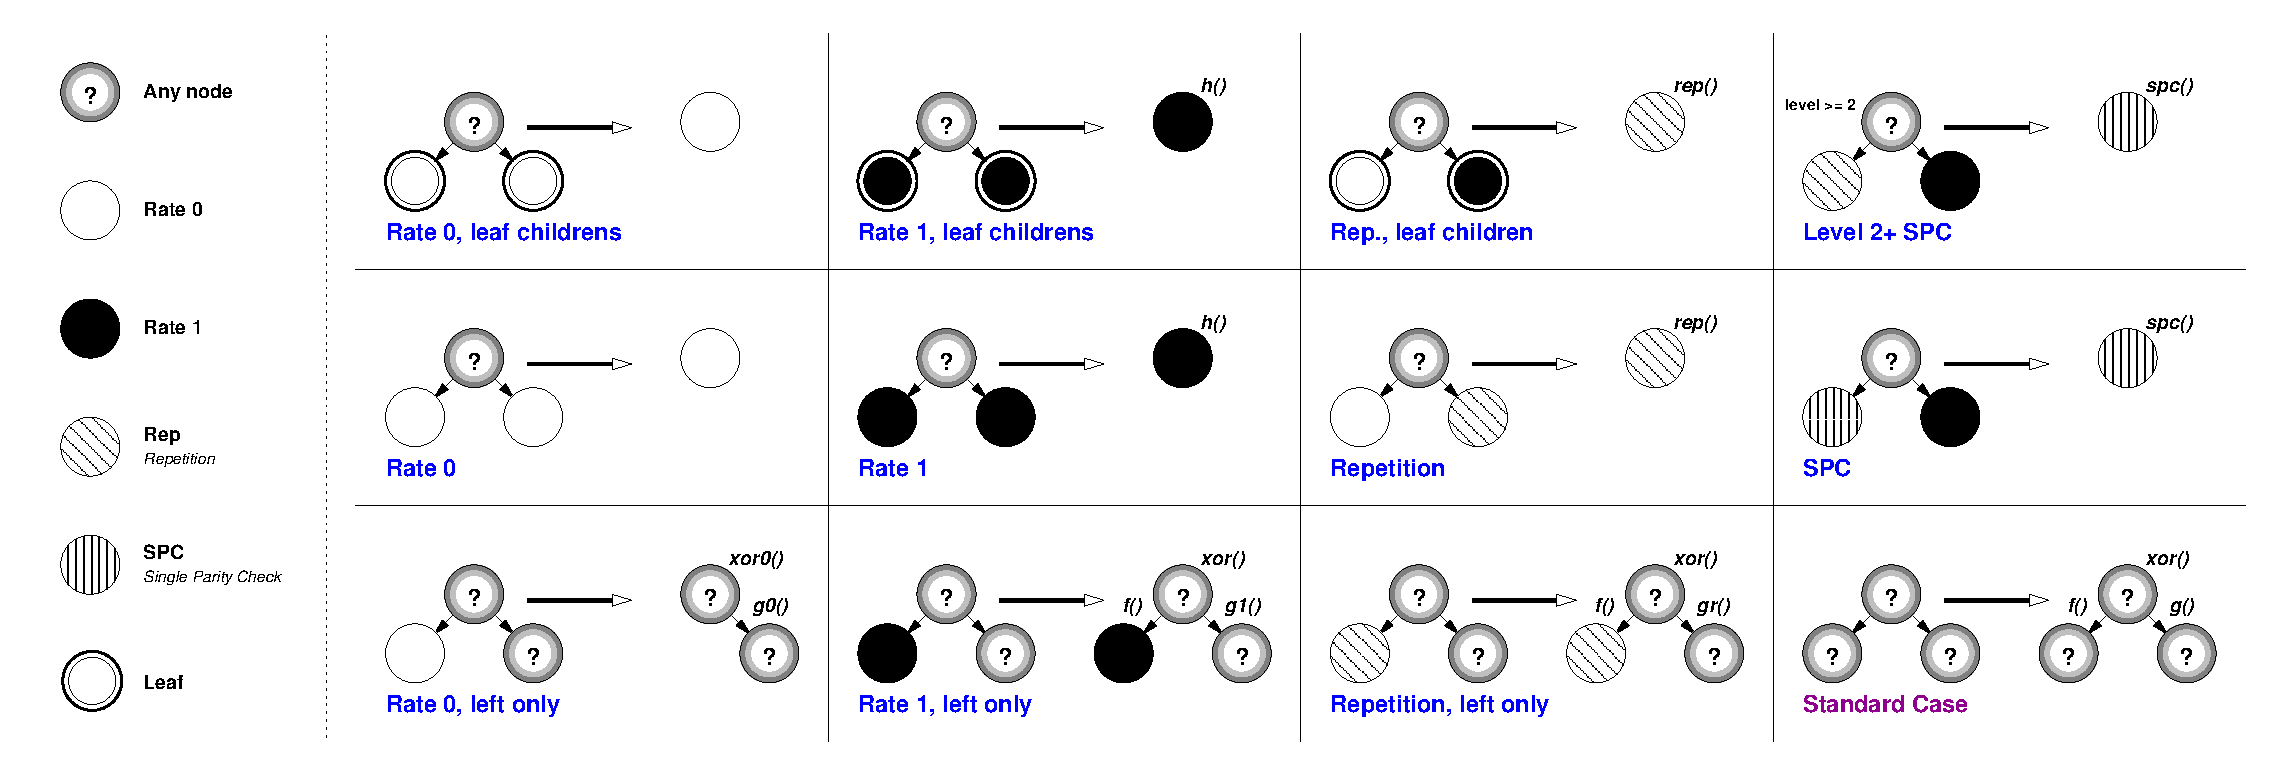
\includegraphics[scale=1.0]{\curChapter/fig/polar/patterns/patterns}
  \caption{Polar sub-tree rewriting rules for processing specialization.}
  \label{fig:opt_polar_patterns}
\end{figure}

For some sub-tree pattern configurations, the processing to be performed at the
root of such sub-trees can be simplified, or even skipped completely, for
instance, when a node only has two frozen bit leaf children. To exploit such
properties, the decoder generator repeatedly applies the set of sub-tree
rewriting rules listed in Figure~\ref{fig:opt_polar_patterns} using a depth
first traversal to alter the node tags, until no rewriting rule applies anymore.

Each rewriting rule defines a subtree pattern \emph{selector}, a new \emph{tag}
for the subtree root, and the $f$, $g$, and $h$ \emph{processing functions} to
be applied, simplified or skipped for this node in the resulting decoder. A
\emph{null} $f$ (resp. $g$) function cuts the left (resp. right) child of the
node. From an implementation point of view, a rule is defined as a class, with a
\verb|match| function and a set of functions $f$, $g$, and $h$. The current
set of rewriting rules can thus easily be enriched with new rules to generate
even more specialized versions.

Patterns on the first two rows result in cutting away both children. For
instance, the first rule cuts the two frozen bit leaf children of the parent
node, and tags it as \verb|R0| (blue node). Processing is completely skipped on
this node since the values of the bits are unconditionally known. The \verb|REP|
rules match subtrees where only the rightmost leaf is black, the others being
frozen bits. In this case, the whole subtree is cut and replaced by a simpler
processing. Moreover a single, specialized $rep$ function is applied on the node
instead of the three functions $f$, $g$ and $h$. The three first rules of the
third line describe partial cuts and specialization. For instance, the third
rule of the third column specializes the $g$ functions in $g_r$, but does not
prune the recursive children processing.

Rewriting rules are ordered by decreasing priority (left to right, then top row
to bottom row in Figure~\ref{fig:opt_polar_patterns}). Thus, if more than one
rule match an encountered subtree, the highest priority rule is applied. The
priority order is chosen such as to favor strongest computation reducing rules
over rules with minor impact, and to ensure confluence by selecting the most
specific pattern first. Rule selectors can match on node tags and/or node levels
(leaf, specific level, above or below some level). A given rule is applied at
most once on a given node.

\subsubsection{Impact of the Tree Pruning on the Decoding Performances}

\begin{figure}[htp]
  \centering
  \subfloat[][32-bit intra-frame SIMD (AVX)]{\includegraphics[width=0.485\textwidth]{\curChapter/fig/polar/sc_tree_cut/sc_tree_cut_intra}\label{plot:opt_polar_sc_tree_cut_intra}}
  \quad
  \subfloat[][8-bit inter-frame SIMD (SSE4.1)]{\includegraphics[width=0.485\textwidth]{\curChapter/fig/polar/sc_tree_cut/sc_tree_cut_inter}\label{plot:opt_polar_sc_tree_cut_inter}}
  \caption
    [Throughput of the SSC decoder depending on the different optimizations.]
    {Throughput of the SSC decoder depending on the different optimizations for
    $N = 2048$, intra-frame vectorization on the left and inter-frame
    vectorization on the right, resp. (on the Intel\R Xeon\TM E31225 CPU).}
  \label{plot:opt_polar_sc_tree_cut}
\end{figure}

The tree pruning step has a dramatical effect in general. For instance, on the
SSC decoder, the reference code for a rate of 1/2 has 2047 nodes, whereas only
291 nodes remain in the pruned version. However, the individual effect of each
rewriting rule is not trivial. The plots in
Figure~\ref{plot:opt_polar_sc_tree_cut} show the specific impact of several
rewriting rules (\verb|R0|, \verb|R1|, \verb|REP| and \verb|SPC|), with
$N = 2048$ and multiple code rates, for intra-frame and inter-frame
vectorization, respectively. The purpose of the plots is to show that no single
rewriting rule dominates for each code rate. They also show that the respective
impact of each rule may vary a lot from rate to rate, making the case for the
flexible, extensible architecture proposed. Indeed, the rewriting rule set can
also be enriched with rules for specific ranges of code rates. For instance, the
rule \emph{Single Parity Check} (\verb|SPC|) has been applied with different
level limits for 9/10 code rate, where it has a significant impact and may
benefit from fine tuning.

\begin{figure}[htp]
  \centering
  \includegraphics[width=0.70\textwidth]{\curChapter/fig/polar/scl_tree_cut/scl_tree_cut}
  \caption
    [Impact of the specialized nodes on the SSCL coded throughput.]
    {Impact of the specialized nodes on the SSCL coded throughput.
    32-bit intra-frame vectorization, $N=2048$ and $L=32$
    (on the Intel\R Core\TM i5-6600K CPU).}
  \label{plot:opt_polar_scl_tree_cut}
\end{figure}

Figure~\ref{plot:opt_polar_scl_tree_cut} shows the impact of the different tree
pruning optimizations on the SSCL decoder throughput according to the code
rate. The performance improvements are cumulative. Coded throughput, in which
the redundant bits are taken into account, is shown instead of information
throughput, for which only information bits are considered. It illustrates the
computational effort without the influence of the fact that higher rate codes
involve higher information throughputs.

The coded throughput of the original unpruned algorithm (\verb|ref|) decreases
as the code rate increases. Indeed, frozen bit leaf nodes are faster to process
than information bit leaf nodes, in which a threshold detection is necessary. As
there are more \verb|R0| and \verb|REP| nodes in low code rates, the tree
pruning is more efficient in the case of low code rates. The same explanation
can be given for \verb|R1| nodes in high code rates. \verb|R1| node pruning is
more efficient than \verb|R0| node pruning on average. Indeed, a higher amount
of computations is saved in \verb|R1| nodes than in \verb|R0| nodes.

It has also been observed in~\cite{Sarkis2016} that when the \verb|SPC| node
size is not limited to $4$, the decoding performance may be degraded.
Consequently the size is limited to $4$ in $\texttt{SPC}_\texttt{4}$. For
$\texttt{SPC}_\texttt{4+}$ nodes, there is no size limit. The two node types are
considered in Figure~\ref{plot:opt_polar_scl_tree_cut}. Therefore, the depth at
which dedicated nodes are activated in the proposed decoder can be adjusted, in
order to offer a tradeoff between throughput and decoding performance.

\begin{figure}[htp]
  \centering
  \includegraphics[width=0.70\textwidth]{\curChapter/fig/polar/scl_spc/scl_spc_diff}
  \caption
    [Effects of the $\texttt{SPC}_\texttt{4+}$ nodes on the CA-SSCL decoder @
     $10^{-5}$ FER]
    {Effects of the $\texttt{SPC}_\texttt{4+}$ nodes on the CA-SSCL decoder @
     $10^{-5}$ FER. 32-bit intra-frame SIMD strategy (on the Intel\R Core\TM
     i5-6600K CPU).}
  \label{plot:opt_polar_scl_spc}
\end{figure}

According to our experiments, the aforementioned statement about performance
degradation caused by $\texttt{SPC}_\texttt{4+}$ nodes is not always accurate
depending on the code and decoder parameters. The impact of switching
\textit{on} or \textit{off} $\texttt{SPC}_\texttt{4+}$ nodes on decoding
performance and throughput at a FER of $10^{-5}$ is detailed in
Figure~\ref{plot:opt_polar_scl_spc}. It shows that $\texttt{SPC}_\texttt{4+}$
nodes have only a small effect on the decoding performance. With $L=8$, an SNR
degradation lower than 0.1 dB is observed, except for one particular
configuration. Throughput improvements from $8$ to $23$ percents are observed.
If $L=32$, the SNR losses are more substantial (up to $0.5$ dB), whereas
throughput improvements are approximately the same. Besides this observation,
Figure~\ref{plot:opt_polar_scl_spc} shows how the proposed decoder flexibility
enables to easily optimize the decoder tree pruning, both for software
implementations and for hardware implementations in which tree pruning can also
be applied~\cite{Lin2014}.

\subsection{Polar Application Programming Interface}
\label{sec:opt_polar_api}

The main challenge in implementing an architecture dependent Application
Programming Interface (API) is to provide enough flexibility to enable varied
types, data layout and optimization strategies such as intra-frame SIMDization
(intra-SIMD) and inter-frame SIMDization (inter-SIMD), without breaking the high
level skeleton abstraction. To meet this requirement, our API heavily relies on
generic programming and compile time specialization by the means of \Cxx
templates, in a manner inspired by \emph{expression template}
techniques~\cite{Stroustrup2013}. Template specializations provide node
functions.

Reducing the decoding time with SIMD instructions is a classical technique in
former software polar decoder implementations. The proposed polar decoders are
based on specific building blocks included from the Polar
API~\cite{Cassagne2015c,Cassagne2016b}. These blocks are fast optimized
implementations of the $f$, $g$, $h$ (and their variants) polar intrinsic
functions defined in Equation~\ref{eq:ctx_polar_f_g_h}.
Listing~\ref{lst:opt_polar_api} details the SIMD implementation of these
functions. These implementations are based on \MIPP. Consequently, the
description is clear, portable, multi-format (32-bit floating-point, 16-bit and
8-bit fixed-points) and as fast as an architecture specific code. The
\verb|mipp::Reg<B>| and \verb|mipp::Reg<R>| types correspond to SIMD registers.
\verb|B| and \verb|R| define the type of the elements that are contained in this
register. \verb|B| for \textit{bit} could be \verb|int|, \verb|short| or
\verb|char|. \verb|R| for \textit{real} could be \verb|float|, \verb|short| or
\verb|char|. In Listing~\ref{lst:opt_polar_api}, each operation is made on
several elements at a time. For instance, line 17, the addition between all the
elements of the \verb|neg_la| and \verb|lb| registers is executed in a single
CPU cycle. We also tried an auto-vectorized approach but even if all the
routines were well vectorized (from the GCC 5.4 compiler report), the
performance was, at least, 3 times slower than the \MIPP handwritten versions.
The template \verb|N_ELMTS| parameter is not used in the proposed
\verb|API_polar_SIMD| implementation. The interest of this parameter will be
explained in the next section.

A single SIMD polar API is necessary to both intra-frame and inter-frame
strategies. In both cases, only the input and output pointers change. The
intra-frame strategy exploits SIMD units without increasing the decoder latency.
Since it still processes frames one at a time, it preserves fine grain
frame pipelining. However, at leaf nodes and nearby, too few elements remain to
fill SIMD units. For instance, 4-way SIMD registers are fully filled only at
level 2 and above. Thus, the intra-frame strategy is only effective on trees
that can be heavily pruned from these numerous scalar nodes. Even if the tree is
heavily pruned some nodes cannot be fully vectorized in the lower layers. In
this context, the building blocks of the polar API enable to automatically
switch from SIMD to sequential implementations.

\begin{listing}
  \inputminted[frame=lines,linenos]{C++}{\curChapter/src/polar/f_g_h_simd.cpp}
  \caption{Example of a \Cxx SIMD polar API ($f$, $g$ and $h$ functions are
    implemented).}
  \label{lst:opt_polar_api}
\end{listing}

\subsection{Successive Cancellation Decoders}
\label{sec:opt_polar_sc}

\subsubsection{Dynamic Implementation}

In this section, if a decoder is generic and flexible, it is called
\emph{dynamic} (as opposed to \emph{generated} or \emph{unrolled} decoders). The
proposed dynamic SSC decoder directly uses the polar API introduced in
Section~\ref{sec:opt_polar_api}. The same source code is able to accommodate
different frozen bit layouts and different parameters ($N$, $K$, SNR). It is the
first non-generated version (to the best of our knowledge) to support both
multi-precisions (32-bit, 16-bit and 8-bit) and multi-SIMD strategies
(intra-frame or inter-frame).

The main challenge of the dynamic SSC decoder is to maintain a good performance
level at the bottom of the tree. Near the leaves, the decoder spends a
non-negligible part of the time in recursive function calls and short loop
executions. In Listing~\ref{lst:opt_polar_api}, the loops lines 6, 15, 23 cannot
be unrolled by the compiler because \verb|n_elmts| is a runtime parameter. Thus,
an useless overhead is due to the loop condition evaluation. To overcome this
problem, we wrote a SSC sub-decoder with the template meta-programming
technique. The idea is to fully unroll the recursive calls and to statically
give the number of elements in the loops lines 6, 15, 23. To this purpose, a
specific \verb|API_polar_SIMD_static| has been developed. The source code is
mainly the same as the \verb|API_polar_SIMD| implementation. The only difference
is that the \verb|n_elmts| parameter has been replaced by the static
\verb|N_ELMTS| parameter in the loops. Then, the compiler is able to unroll
the loops. The size of the unrolled sub-tree can be adjusted from a static
parameter in the source code. We found that a sub-tree with a depth of 6 gives
a good level of performance. Increasing the size of the sub-tree to more than 6
did not give any performance gains in our tests. As a consequence, the proposed
flexible decoder cannot decode polar codes smaller than $N = 2^6 = 64$. This is
acceptable knowing that the error-rate performance of the SSC decoder is good
for large frame sizes.

To go even further and reach highest throughputs and lowest latencies possible,
the next section proposes to fully unroll/generate the SSC decoder.

\subsubsection{Unrolled/Generated Implementation}
\label{sec:opt_polar_pedge}

\paragraph{Specialized Decoder Skeletons and Polar API}

The tree structure at the heart of SC decoders is fully determined by the
parameters of a given polar code instance: the code size, the code rate ($R = K
/ N$), the position of the frozen bits. All these parameters are  statically
known at compile time. Yet, the recursive tree traversal code structure and the
corresponding tree data structure are challenging to vectorize and to optimize
for a compiler. Our Polar ECC Decoder Generation Environment (P-EDGE) builds on
this property to provide a general framework for polar decoder design,
generation and optimization\footnote{P-EDGE repository: \url{https://github.com/aff3ct/polar_decoder_gen}}.
Beyond the \emph{code parameters}, Polar decoders
can be tweaked and optimized in many different orthogonal or loosely coupled
ways: \emph{Elementary} type (floating-point, fixed-point),
\emph{Element containers} (array size), \emph{Data layout} (bit packing
techniques), \emph{Instruction Set} (x86, ARM\R), \emph{SIMD} support (scalar,
intra-frame or inter-frame processing vectorization), \emph{SIMD instruction set
variant} (SSE, AVX, AVX-512, NEON), as well as the set and relative priorities
of the \emph{rewriting rules for tree pruning}. Our framework enables to quickly
experiment the different combinations of all optimizations. Thus, the decoder
description results from two distinct parts:
\begin{itemize}
  \item An architecture independent \emph{specialized decoder skeleton}
    generated by our decoder generator, from a given frozen bits location input.
    Starting from the naive, recursive expression of the computational tree, we
    apply successively cuts and specializations on the tree. They are described
    through a set of rewriting rules, that can be customized according to the
    specificities of the decoder and to the constraints in terms of code size
    for instance (see Section~\ref{sec:opt_polar_pattern_matching}).
  \item A library of architecture dependent \emph{elementary computation
    building blocks}, corresponding to the implementation variants of the $f$,
    $g$ and $h$ functions (fixed- or floating-point versions, scalar or vector
    versions, ...). These blocks do not depend on the frozen bits location and
    can therefore be used by any specialized skeleton (see
    Section~\ref{sec:opt_polar_api}).
\end{itemize}

This separation of concerns, between high-level specialized algorithmic
skeletons and low-level arithmetic routines, enables both ECC experts to focus
on optimizing algorithm skeletons and architecture experts to focus on writing
highly optimized routines.

\newpage
\paragraph{Decoder Generation}

\begin{listing}[htp]
  \inputminted[frame=lines,linenos]{C++}{\curChapter/src/polar/generated_sc_decoder.cpp}
  \caption
    [Generated polar SC decoder source code.]
    {Generated polar SC decoder source code corresponding to the pruned tree in
     Figure~\ref{fig:ctx_polar_tree_pruning_example}.}
  \label{lst:opt_polar_generated_sc_decoder}
\end{listing}

The decoder generator first builds the binary tree structure from the pattern
matching algorithm presented in Section~\ref{sec:opt_polar_pattern_matching}.
Then, once the tree has been fully specialized, the P-EDGE generator performs a
second tree traversal pass to output the resulting decoder. An example of such a
tree specialization process together with the generator output is shown in
Figure~\ref{fig:ctx_polar_tree_pruning_example} and in
Listing~\ref{lst:opt_polar_generated_sc_decoder}. In
Listing~\ref{lst:opt_polar_generated_sc_decoder}, each operation (\verb|f|,
\verb|rep|, \verb|gr|, \verb|spc| and \verb|h|) is applied on $4$ elements. This
number of elements is given as a static template parameter as well as a standard
function parameter. Depending on the selected polar API, one or the other will
be used. Of course with fully unrolled decoders, it is much more efficient to
use an API implementation that uses the template parameter to fully unroll the
loops at compile time.

\paragraph{Source Code Compression}
\label{sec:opt_polar_sc_compression}

\begin{figure}[htp]
  \centering
  \subfloat[][Legend.]{
    \includegraphics{\curChapter/fig/polar/sc_gen_compression/sc_gen_compression_legend}
  }
  \\
  \subfloat[][Without compression.]{
    \label{fig:opt_polar_sc_gen_compression_wo}
    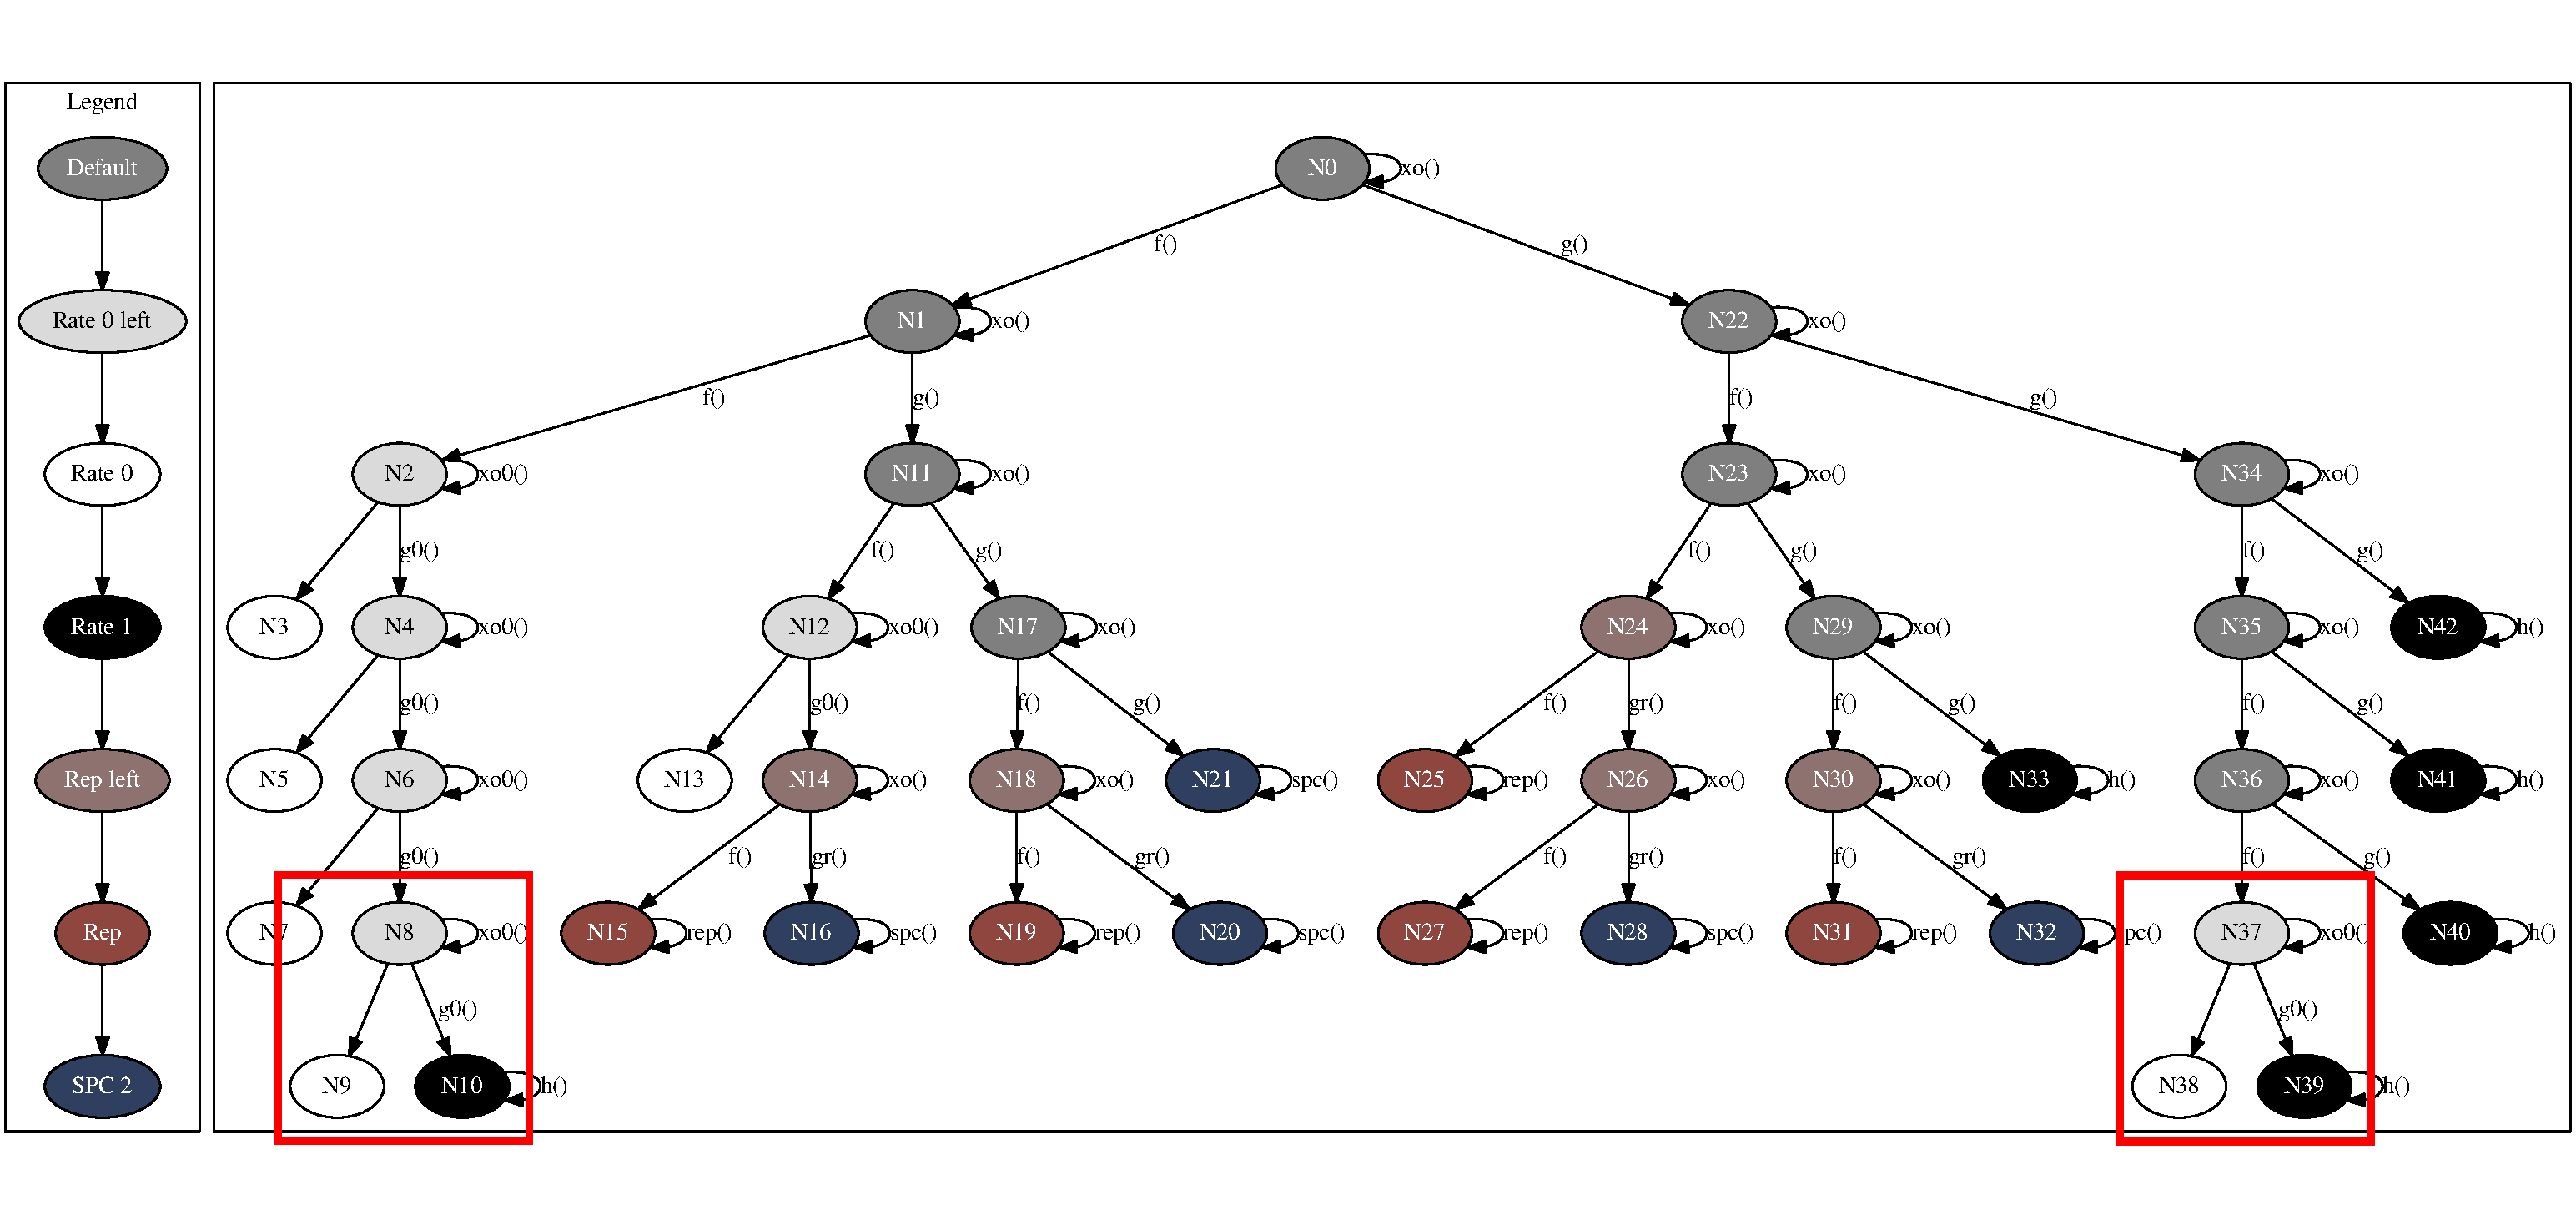
\includegraphics{\curChapter/fig/polar/sc_gen_compression/sc_gen_no_compression}
  }
  \\
  \subfloat[][With compression.]{
    \label{fig:opt_polar_sc_gen_compression_w}
    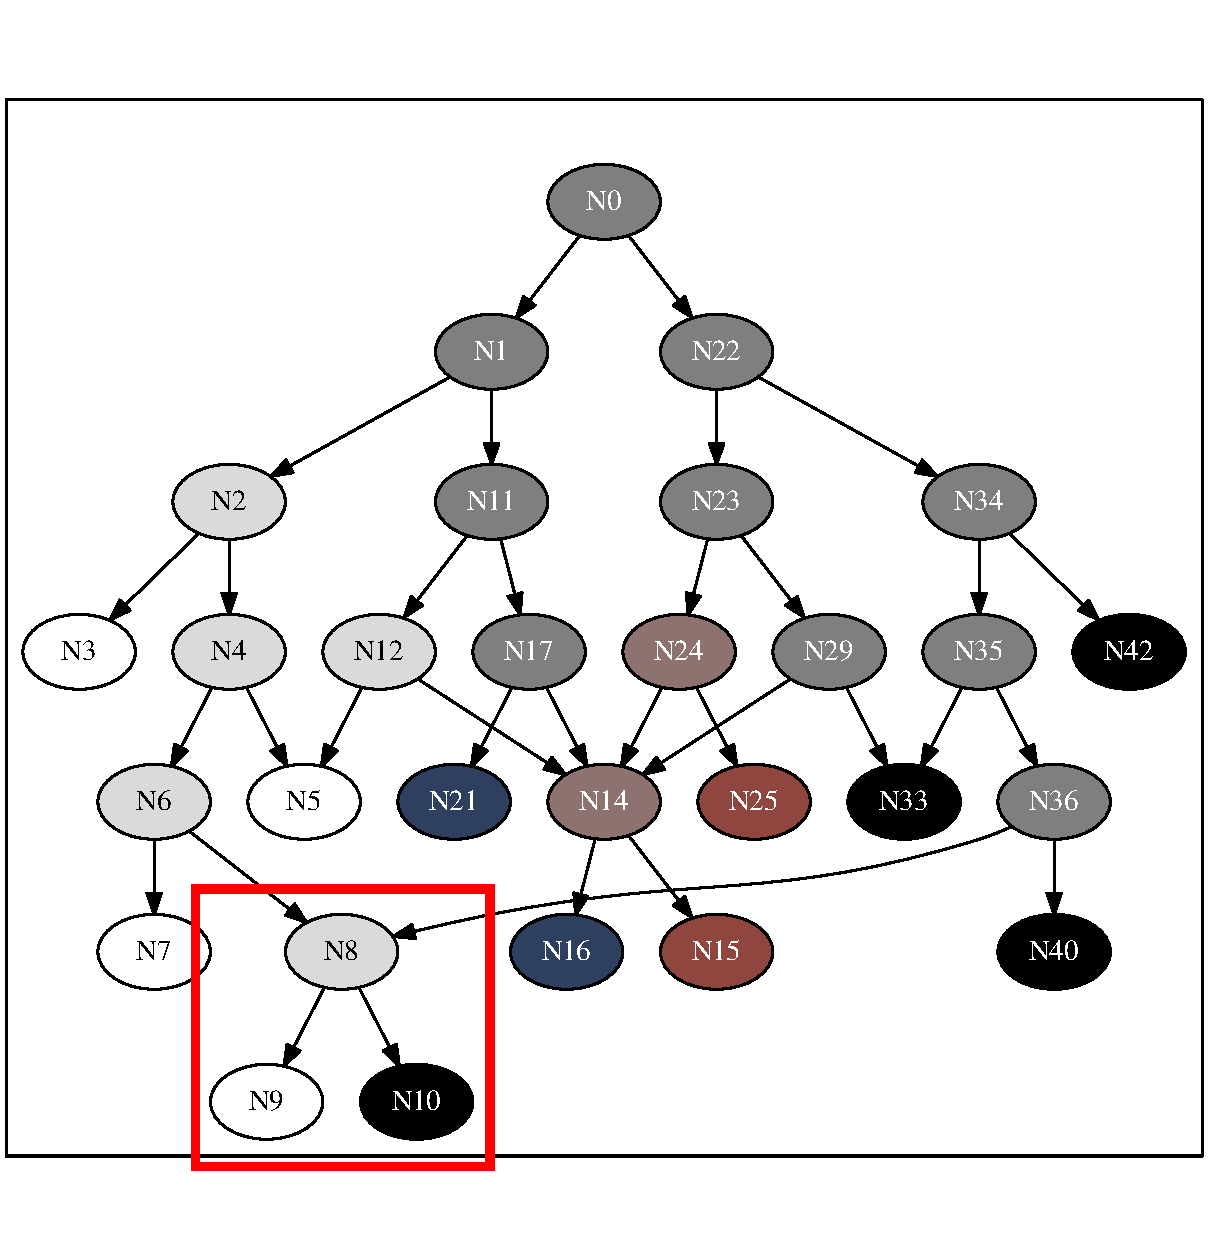
\includegraphics{\curChapter/fig/polar/sc_gen_compression/sc_gen_compression}
  }
  \caption
    [Pruned polar decoding tree representation without and with compression.]
    {Pruned polar decoding tree representation ($N = 128, K = 64$) without
    and with the compression sub-tree folding algorithm.}
  \label{fig:opt_polar_sc_gen_compression}
\end{figure}

Decoders are generated as straight-line code (no recursive calls), with all node
computations put in sequence. This improves performance for small to medium
codeword sizes, up to the point where the compiled binary exceeds the L1I cache
size (this is also reported in~\cite{Giard2016b}). We mitigated this issue by
reducing decoder binary sizes using two compression techniques: 1) in the
generated code, we moved the buffer offsets from template arguments to function
arguments, which enabled the compiler to factorize more function calls than
before (improvement by a factor of 10), 2) we implemented a sub-tree folding
algorithm in the P-EDGE generator (see
Figure~\ref{fig:opt_polar_sc_gen_compression}), to detect multiple occurrences
of a same sub-tree and to put the corresponding code into a dedicated function.
These techniques lead to an improvement by a factor of 5 for $N=2^{16}$ knowing
that the compression ratio increases with the size of the tree.

\newpage
\subsubsection{LLRs and Partial Sums Memory Management}

The memory management is similar in the flexible SSC decoder and in the unrolled
versions. Each time, the decoder stores its state using two data buffers, one
for the LLR values ($\bm{\lambda}$) and the other for the bits (partial sums
$\bm{\hat{s}}$). The ``logical'' tree layout is implemented as a simple and
efficient \emph{heap} vector data layout. Therefore traversing the tree
corresponds to moving through the array, at different offsets and considering
different index intervals. The LLR offset is computed from the graph depth~$d$
(the node vertical indexing) as follows:
\begin{equation}
 o_{\lambda}(d) = \begin{cases}
   0                                         &\text{$d = 0$},\\
   \sum\limits_{i = 1}^{d} \frac{N}{2^{i-1}} &\text{otherwise.}
\end{cases}
\end{equation}
Given~$l_a$ the lane (the node horizontal indexing), the bit offset is
determined as follows:
\begin{equation}
  o_{\hat{s}}(d,l_a) = \frac{N}{2^d} \times l_a.
\end{equation}
The LLR buffer size is $2N$ and the bit buffer is $N$, for a frame of $N$ bits.
Thus, the memory footprint per frame can be expressed:
\begin{equation}
  mem_{fp} = N \times (2 \times \sizeof(LLR) + \sizeof(bit)).
\end{equation}
LLRs element size is 4 bytes (float) or 1 byte (fixed-point numbers). The
inter-SIMD version also employs a \emph{bit packing} memory footprint reduction
technique~\cite{LeGal2015a} to pack several bits together by using shifts and
masking instructions.

\subsection{Successive Cancellation List Decoders}
\label{sec:opt_polar_scl}

In this section, the proposed implementation of the SSCL class of decoders
focuses on intra-frame SIMD dynamic decoders. A description of a fully unrolled
SSCL decoder has been previously evaluated in~\cite{Sarkis2016}. But, we want to
oppose it to more generic and flexible decoders. Some implementation
improvements are necessary in order to be competitive with specific unrolled
decoders of the literature. The polar API (see Section~\ref{sec:opt_polar_api})
enables to benefit from the SIMD instructions for various target architectures.
Optimizations of CRC checking benefit to both the non-adaptive and adaptive
versions of the CA-SSCL algorithms. The new sorting technique presented in
Section~\ref{sec:opt_polar_scl_sorting} can be applied to each variation of the
SSCL algorithm. Finally, an efficient implementation of the partial sums memory
management is proposed in Section~\ref{sec:opt_polar_scl_partial_sum}. It is
particularly effective for short polar codes.

\subsubsection{Improving Cyclic Redundancy Checking}
\label{sec:opt_polar_scl_crc}

By profiling the Adaptive SCL decoder, one may observe that a significant amount
of time is spent to process the cyclic redundancy checks. Its computational
complexity is O($LN$) versus the computational complexity of the SCL decoding,
O($LN\log N$). The first is not negligible compared to the second. In the
adaptive decoder, the CRC verification is performed a first time after the SC
decoding. In the following, we show how to reduce the computational complexity
of these CRC verifications.

\newpage
First, an efficient CRC checking code has been implemented. Whenever the decoder
has to check the CRC, the bits are packed and then computed 32 by 32. In order
to further speed up the implementation, a lookup table used to store
pre-computed CRC sub-sequences, and thus reduce the computational complexity.
The size of the lookup table is 1 KB.

After a regular SC decoding, a decision vector of size $N$ is produced. Then,
the $K$ information bits must be extracted to apply cyclic redundancy check. The
profiling of our decoder description shows that this extraction takes a
significant amount of time compared to the check operation itself. Consequently,
a specific extraction function was implemented. This function takes advantage of
the leaf node type knowledge to perform efficient multi-element copies.

Concerning SCL decoding, it is possible to sort the candidates according to
their respective metrics and then to check the CRC of each candidate from the
best to the worst. Once a candidate with a valid CRC is found, it is chosen as
the decision. This method gives similar decoding performance as performing the
CRC of each candidate and then selecting the one with the
best metric. With the adopted order, decoding time is saved by reducing the
average number of checked candidates. This is made in the
``$\selectBestPath()$'' sub-routine (Algorithm~\ref{alg:ctx_polar_scl_decoder},
l.18).

\subsubsection{LLR and Metric Sorting}
\label{sec:opt_polar_scl_sorting}

Metric sorting is involved in the path selection step, but also
in the ``$\updatePaths()$'' sub-routine
(Algorithm.~\ref{alg:ctx_polar_scl_decoder}, l.16) and consequently in each
leaf. Sorting the LLRs is also necessary in \verb|R1| and \verb|SPC| nodes.
Because of a lack of information about the sorting technique presented
in~\cite{Sarkis2016}, its reproduction is not possible. In this paragraph, the
sorting algorithm used in our proposed SCL decoder is described.

In \verb|R1| nodes, a Chase-$2$~\cite{Chase1972} algorithm is applied. The two
minimum absolute values of the LLRs have to be identified. The way to do the
minimum number of comparisons to identify the $2$ largest of $n\geq2$ elements
was originally described by Schreier in~\cite{Schreier1932} and reported
in~\cite{Knuth1973}. The lower stages of this algorithm can be parallelized
thanks to SIMD instructions in the way described in~\cite{Furtak2007}. According
to our experimentations, Schreier's algorithm is the most efficient compared to
parallelized Batcher's merge exchange, partial quick-sort or heap-sort
implemented in the \Cxx standard library in the case of \verb|R1| nodes. At the
end, we chose not to apply the SIMD implementation of Schreier's algorithm
because: 1) the speedup was negligible, 2) in 8-bit fixed-point, only
$N \leq 256$ codewords can be considered.

Concerning path metrics, partial quick-sort appeared to yield no gains in terms
of throughput by comparison with the algorithm in~\cite{Schreier1932}, neither
did heap-sort or parallelized Batcher's merge exchange. For a matter of
consistency, only Schreier's algorithm is used in the proposed decoder, for both
LLR sorting in \verb|R1| and \verb|SPC| nodes and for path metrics sorting. The
sorting of path metrics is applied to choose the paths to be removed, kept or
duplicated.

\subsubsection{Partial Sums Memory Management}
\label{sec:opt_polar_scl_partial_sum}

An SCL decoder can be seen as $L$ replications of an SC decoder. The first
possible memory layout is the one given in
Figure~\ref{fig:ctx_polar_sc_decoder}. In this layout, the partial sums
$\hat{s}$ of each node is stored in a dedicated array. Therefore, a memory of
size $2N-1$ bits is necessary in the SC decoder, or $L(2N -1)$ bits in the SCL
decoder. This memory layout is described in~\cite{Tal2011} and present in
previous software implementations~\cite{Sarkis2014b,Sarkis2016,Shen2016}.

A possible improvement is to change the memory layout to reduce its footprint.
Due to the order of operations in both SC and SCL algorithms, the partial sums
on a given layer are only used once by the $h$ function and can then be
overwritten. Thus, a dedicated memory allocation is not necessary at each layer
of the tree. The memory can be shared between the stages. Therefore the memory
footprint can be reduced from $2N-1$ to $N$ in the SC decoder as shown
in~\cite{Leroux2013}. A reduction from $L(2N -1)$ to $LN$ can be obtained in the
SCL decoder.

In the case of the SCL algorithm, $L$ paths have to be assigned to $L$ partial
sum memory arrays. In~\cite{Tal2011}, this assignment is made with pointers. The
advantage of pointers is that when a path is duplicated, in the
``$\updatePaths()$'' sub-routine of Algorithm~\ref{alg:ctx_polar_scl_decoder},
the partial sums are not copied. Actually, they can be shared between paths
thanks to the use of pointers. This method limits the number of memory
operations. Unfortunately, it is not possible to take advantage of the memory
space reduction. Indeed, the partial sums have to be stored on $L(2N -1)$ bits.
There is an alternative to this mechanism. If a logical path is statically
assigned to a memory array, no pointer is necessary at the cost that partial
sums must be copied when a path is duplicated (only $LN$ bits are required).
This method is called SSCL$_{\texttt{cpy}}$ whereas the former is called
SSCL$_{\texttt{ptr}}$.

\begin{figure}[htp]
  \centering
  \includegraphics[width=0.70\textwidth]{\curChapter/fig/polar/scl_cpy_vs_ptr/scl_cpy_vs_ptr}
  \caption
    [Throughput of the SSCL decoder depending on the partial sums management.]
    {Information throughput of the SSCL decoder depending on the codeword
    size ($N$) and the partial sums management. $R = 1 / 2$, $L = 8$ (on the
    Intel\R Core\TM i5-6600K CPU).}
  \label{plot:opt_polar_scl_cpy_vs_ptr}
\end{figure}

Our experiments have shown that the overhead of handling pointers plus the
extra memory space requirement cause the SSCL$_{\texttt{cpy}}$ to be more
efficient than the SSCL$_{\texttt{ptr}}$ for short and medium code lengths, as
shown in Figure~\ref{plot:opt_polar_scl_cpy_vs_ptr}. The 32-bit version uses
floating-point LLRs, whereas 16-bit and 8-bit versions are in fixed-point.
Notice that in this work, each bit of the partial sums is stored as an 8-bit,
16-bit or 32-bit number accordingly to the LLR data type. The code rate $R$ is
equal to $1/2$. The throughput of the SSCL$_{\texttt{cpy}}$ version is higher
for $N \leq 8192$ whereas the SSCL$_{\texttt{ptr}}$ version is more efficient
for higher values of $N$. Figure~\ref{plot:opt_polar_scl_cpy_vs_ptr} also
illustrates the impact of the representation of partial sums. For very high
values of $N$, the 8-bit fixed point representation takes advantage of fewer
cache misses. As the decoding performance improvements of the SCL algorithm are
not very significant compared to the SC algorithm for long polar codes,
SSCL$_{\texttt{cpy}}$ is the appropriate solution in most practical cases.

In our decoder description, LLRs are managed with pointers, as it is the case in
other software implementations of the literature~\cite{Sarkis2014b,Sarkis2016,
Shen2016}. We tried to remove the pointer handling as for the partial sums, but
this was not beneficial in any use case.

\subsubsection{Memory Footprint}

\begin{table}[htp]
  \centering
  \caption{Polar decoders memory complexity.}
  \label{tab:opt_polar_scl_memory_footprint}
  \begin{tabular}{r r}
    \textbf{Algorithms}        & \textbf{Memory Footprint} \\
    \hline
    \hline
    (CA-)SSCL$_{\texttt{cpy}}$ & $\mathcal{O}((2L + 1)NQ)$ \\
    (CA-)SSCL$_{\texttt{ptr}}$ & $\mathcal{O}((3L + 1)NQ)$ \\
    A-SSCL$_{\texttt{cpy}}$    & $\mathcal{O}((2L + 3)NQ)$ \\
    A-SSCL$_{\texttt{ptr}}$    & $\mathcal{O}((3L + 3)NQ)$ \\
 \end{tabular}
\end{table}

The exact memory footprint of the SSCL decoders is hard to estimate as there are
many small buffers related to the implementation. However, the memory footprint
is mainly driven by the LLRs ($\bm{\lambda}$) and the partial sums
($\bm{\hat{s}}$) as they linearly depend on $LN$. The buffers related to the
path metrics can be neglected as they linearly depend on $L$. The memory
footprint of the CRC is also negligible, the only requirement is a lookup table
of 256 integers. Table~\ref{tab:opt_polar_scl_memory_footprint} summarizes the
memory footprint estimation of the various decoders while $Q$ stands for the
size of the element (1, 2 or 4 bytes). The channel LLRs are taken into account
in the approximation. As explained in the previous section, the
SSCL$_{\texttt{ptr}}$ version of the code requires twice the amount of data for
the partial sums. Notice that the memory footprint of the adaptive decoders is a
little bit higher than the other SSCL decoder since it includes an additional
SSC decoder.

In this section we proposed flexible software implementations of the SC and the
SCL decoding algorithms. The pruned versions of these decoders (SSC and SSCL)
are the key of efficiency. The generated (or unrolled) strategy has also been
experimented and improved for the SSC decoders. These specialized decoders trade
a part of the flexibility for higher throughput and lower latency performance.

\section{Turbo Decoders}

A turbo decoder is in charge of decoding a large set of frames. Two strategies
are then possible to speedup the decoding process. i)
\textit{intra-frame parallelism}: the decoder exploits the parallelism within
the turbo-decoding process by executing concurrent tasks during
the decoding of one frame. ii) \textit{inter-frame parallelism}: several frames
are decoded simultaneously. In the perspective of a hardware implementation, the
intra-frame approach is efficient~\cite{Muller2009} because the area overhead
resulting from parallelization is lower than the speedup. On the contrary, the
inter-frame strategy is inefficient, due to the duplication of multiple hardware
turbo-decoders. The resulting speedup comes at a high cost in terms of area
overhead.

In the perspective of a software implementation, the issue is different. The
algorithm is executed on a programmable non-modifiable architecture. The degree
of freedom lies in the mapping of the different parallelizable tasks on the
parallel units of the processor. Modern multi-core processors support Single
Program Multiple Data (SPMD) execution. Each core includes Single Instruction
Multiple Data (SIMD) units. The objective is then to identify the
parallelization strategy suitable for both SIMD and SPMD programming models.
In the literature, intra-frame parallelism is often mapped on SIMD units while
inter-frame parallelization is usually kept for multi-threaded approaches
(SPMD). In~\cite{Zhang2012,Wu2013}, multiple trellis-state computations are
performed in parallel in the SIMD units. In~\cite{Wu2010,Wu2011,Chinnici2012,
Yoge2012,Zhang2012,Liu2013,Chen2013,Xianjun2013,Wu2013,Zhang2014,Li2014}, the
decoded frame is split into sub-blocks that are processed in parallel in the
SIMD units. An alternative approach is to process both SISO decoding in
parallel but, it requires additional computations for synchronization and/or
impacts on error-correction performance~\cite{Muller2009}. However, for all
these approaches a part of the computation of the BCJR decoder remains
sequential, bounding the speedup below the capabilities of SIMD units.
Inter-frame parallelism has been proposed in~\cite{Wu2010,Wu2011,Zhang2012,
Wu2013}. Multiple codewords are decoded in parallel, this improves the memory
access regularity and the usage rate of SIMD units. The speedup is no longer
bounded by the sequential parts, all removed, but this comes at the expense of
an increase in memory footprint and latency.
In this work, we focus on the inter-frame parallelization and show that the use
of this approach enables some register-reuse optimizations that are not possible
in the intra-frame strategy.

\subsection{Inter-frame Parallelism on Multi-core CPUs}

The contribution of this work is to propose an efficient mapping of multiple
frames on the CPU SIMD units (inter-frame strategy): the decoding of $F$ frames
is vectorized. Before the decoding process can be launched, this new approach
requires to: (a) buffer a set of $F$ frames and (b) reorder the input LLRs in
order to make the SIMDization efficient with memory aligned operations (see
Section~\ref{sec:opt_vec_inter}). Similarly, a reverse-reordering step has to be
performed at the end of the turbo decoding. These reordering operations are
expensive but they make the complete decoding process very regular and efficient
for SIMD parallelization. Moreover, reordering is applied only once,
independently of the number of decoding iterations.

\begin{algorithm}
  \caption{Loop fusion BCJR implementation.}
  \label{alg:opt_turbo_bcjr_loop_fusion}

  \For(\Comment*[f]{Vectorized loop}){all frames}
  {
    $\boldsymbol{\alpha}^0\gets \initAlpha()$

    \For(\Comment*[f]{Sequential loop}){$k=1;~k<K;~k=k+1$}
    {
      $\boldsymbol{\gamma}^{k-1}\gets \computeGamma(L_{s}^{k-1}, L_{p}^{k-1}, L_{a}^{k-1})$

      $\boldsymbol{\alpha}^k\gets \computeAlpha(\boldsymbol{\alpha}^{k-1}, \boldsymbol{\gamma}^{k-1})$
    }

    $\boldsymbol{\gamma}^{K-1}\gets \computeGamma(L_{s}^{K-1}, L_{p}^{K-1}, L_{a}^{K-1})$

    $\boldsymbol{\beta}^{K-1}\gets \initBeta()$

    $L_e^{K-1}\gets \computeExtrinsic(\boldsymbol{\alpha}^{K-1}, \boldsymbol{\beta}^{K-1}, \boldsymbol{\gamma}^{K-1}, L_{s}^{K-1}, L_{a}^{K-1})$

    \For(\Comment*[f]{Sequential loop}){$k=K-2;~k \geq 0;~k=k-1$}
    {
      $\boldsymbol{\beta}^k\gets \computeBeta(\boldsymbol{\beta}^{k+1}, \boldsymbol{\gamma}^{k})$

      $L_e^{k}\gets \computeExtrinsic(\boldsymbol{\alpha}^{k}, \boldsymbol{\beta}^k, \boldsymbol{\gamma}^{k}, L_{s}^{k}, L_{a}^{k})$
    }
  }
\end{algorithm}

In the proposed implementation, the inter-frame parallelism is used to fill the
SIMD units of the CPU cores. Algorithm~\ref{alg:ctx_turbo_bcjr} illustrates the
traditional implementation of the BCJR (used for the \emph{intra-frame}
vectorization). The inter-frame strategy makes the outer loop on the frame
parallel (through vectors). This means all computations inside this loop operate
on SIMD vectors instead of scalars. The inner loops can be turned into
sequential loops on SIMD vectors. This gives the opportunity for memory
optimizations, through loop fusion. The initial 4 inner loops are merged into 2
loops. Algorithm~\ref{alg:opt_turbo_bcjr_loop_fusion} presents this loop fusion
optimization. This makes possible the scalar promotion of $\beta_j$ (no longer
an array). Indeed, it can be directly reused from the CPU registers. In this
version, the SIMD are always stressed.

On a multi-core processor, each core decodes $F$ frames using its own SIMD unit.
As $T$ threads are activated, a total of $F\times T$ frames are therefore
decoded simultaneously with the inter-frame strategy. Theoretically, this SPMD
parallelization strategy provides an acceleration up to a factor~$T$, with $T$
cores. Large memory footprint exceeding L3 cache capacity may reduce the
effective speedup, as shown in Section~\ref{sec:eval_turbo}.

\subsection{Software Implementation of the Turbo Decoder}
\label{sec:opt_turbo_implem}

\subsubsection{Fixed-point Representation}

Nowadays on x86 CPUs, there are large SIMD registers: SSE/NEON are 128 bits
wide and AVX are 256 bits wide. The number of elements that can be vectorized
depends on the SIMD length and on the data format:
$p_\text{SIMD} = \sizeof(\text{SIMD}) / \sizeof(\text{data})$. So, the key for a
wide parallelism is to work on short data.

During the turbo-decoding process, the extrinsic values grow at each iteration.
It is then necessary for internal LLRs to have a larger dynamic than the channel
information. Depending on the data format, 16-bit or 8-bit, the quantization
used in the decoder is $Q_{16,3}$ or $Q_{8,2}$, respectively.

\subsubsection{Memory Allocations}

The systematic information $\bm{L_s}$/$\bm{L'_s}$ and the parity information
$\bm{L_p}$/$\bm{L'_p}$ are stored in the natural domain $\mathcal{N}$ as well as
in the interleaved domain $\mathcal{I}$. Moreover, two extrinsic vectors are
stored: $\bm{L_{e:1 \rightarrow 2}}$ in $\mathcal{N}$ and
$\bm{L_{e:2 \rightarrow 1}}$ in $\mathcal{I}$ as well as two a priori vectors:
$\bm{L_{a:1 \rightarrow 2}}$ in $\mathcal{I}$ and
$\bm{L_{a:2 \rightarrow 1}}$ in $\mathcal{N}$. Inside the BCJR decoding and per
trellis section, two $\gamma_{i}$ and eight $\alpha_{j}$ metrics are stored.
Thanks to the loop fusion optimization, the eight $\beta_j$ metrics are not
stored in memory. In the proposed implementation $i \in \{0,1\}$ and $j \in
\{0,1,2,3,4,5,6,7\}$. Notice that all those previously-mentioned vectors are
$K$-bit wide and are duplicated $F\times T$ times because of the inter-frame
strategy. The memory footprint in bytes is approximately: $18 \times K \times
\sizeof(\text{data}) \times F \times T$ (where $F = p_\text{SIMD}$). The
interleaving and deinterleaving lookup tables have been neglected in this model.

\subsubsection{Forward Trellis Traversal}

The objective is to reduce the number of loads/stores by performing the
arithmetic computations (\verb|add| and \verb|max|) inside registers. The
max-log-MAP (ML-MAP) algorithm only stresses the integer pipeline of the CPU.
This kind of operations takes only one cycle to execute when the latency is also
very small (1 cycle too). In contrast, a load/store can take a larger number of
cycles depending on where the current value is loaded/stored in the memory
hierarchy. Using data directly from the registers is cost-free but
loading/storing it from the L1/L2/L3 cache can take up to 30 cycles (at worst).

Per trellis section $k$, the two $\gamma_i^k$ metrics are computed from the
systematic and the parity information. These two $\gamma_i^k$ are directly
reused to compute the eight $\alpha_j^k$ metrics. Depending on the number of
bits available, the trellis traversal requires to normalize the $\alpha_j^k$
because of the accumulations along the multiple sections.  In 8-bit format, the
$\alpha_j^k$ metrics are normalized for each section: the first $\alpha_0^k$
value is subtracted from all the $\alpha_j^k$ (including $\alpha_0^k$ itself).
In the 16-bit decoder, the normalization is only applied every eight steps,
since there are enough bits to accumulate eight values. We have observed in
experiments that there is no performance degradation due to the normalization
process. At the end of a trellis section $k$ the two $\gamma_i^k$ and the eight
normalized $\alpha_j^k$ are stored in  memory. In the next trellis section
($k+1$) the eight previous $\alpha_j^k$ are not loaded from memory but they are
directly reused from registers to compute the $\alpha_j^{k+1}$ values.

\subsubsection{Backward Trellis Traversal}

Per trellis section $k$, the two $\gamma_i^k$ metrics are loaded from the
memory. These two metrics are then used to compute, on the fly, the eight
$\beta_j^k$ metrics (whenever needed the $\beta_j^k$ metrics have been
normalized like for the $\alpha_j^k$ metrics). After that, the $\alpha_j^k$
metrics are loaded from the memory. The $\alpha_j^k$, $\beta_j^k$ and
$\gamma_i^k$ metrics are used to determine the \textit{a posteriori} and the
extrinsic LLRs. In the next trellis section ($k-1$) the previous $\beta_j^k$
metrics are directly reused from registers in order to compute the next
$\beta_j^{k-1}$ values. The $\beta_j^k$ metrics are never stored in memory.

\subsubsection{Loop Unrolling}

\begin{listing}[htp]
  \inputminted[frame=lines,linenos]{C++}{\curChapter/src/turbo/alpha_generic.cpp}
  \caption
    [Generic implementation of the BCJR $\bm{\alpha^k}$ computations.]
    {Generic implementation of the $\bm{\alpha^k}$ computations.}
  \label{lst:opt_turbo_alpha_generic}
\end{listing}

\begin{listing}[htp]
  \inputminted[frame=lines,linenos]{C++}{\curChapter/src/turbo/alpha_unrolled.cpp}
  \caption
    [Unrolled implementation of the BCJR $\bm{\alpha^k}$ computations.]
    {Unrolled implementation of the $\bm{\alpha^k}$ computations.}
  \label{lst:opt_turbo_alpha_unrolled}
\end{listing}

The computations of the eight $\alpha^k_j$ states can be implemented with
a generic \verb|trellis| structure as shown in
Listing~\ref{lst:opt_turbo_alpha_generic}. The main problem is that the loop
line 1 cannot be unrolled by the compiler and there is extra memory accesses (or
indirections) due to the \verb|trellis| vector. Knowing precisely the structure
of the trellis in the LTE standard (see Figure~\ref{fig:ctx_turbo_encoder_lte}),
it is possible to fully unroll the loop. The unrolled description is shown in
Listing~\ref{lst:opt_turbo_alpha_unrolled}. This version is adopted in
the Section~\ref{sec:eval_turbo} as it leads to significant throughput
improvements. The same optimization is also applied to the computation of the
$\beta^k_j$ states. One can note that the source code examples are simplified:
\verb|gamma| represents the corresponding $\gamma^k_i$.

In this section, we presented a high throughput implementation of the turbo
decoding algorithm. This implementation largely relies on the inter-frame SIMD
strategy combined with a fixed-point representation of the LLRs and some
specializations for the LTE 8-state trellis.

\section{SCMA Demodulators}
\label{sec:opt_scma}

Besides methodical improvements of the MPA such as log-MPA, hardware oriented
improvements are important to take full benefit of C-RAN servers
capabilities. Since MPA and log-MPA are control heavy algorithms, mishandling of
data can induce huge performance losses. This section explores how MPA can be
reformulated: 1) to improve data locality in cache and to reduce cache misses
and branch mispredictions 2) to reorder the data paths in order to help
exploiting data-level parallelism at each step of the MPA and log-MPA algorithms
and 3) to exploit approximated modeling of additive white Gaussian noise in
order to eliminate exponential calculations and to drastically reduce the number
of SIMD instructions.

\subsection{Flattening Matrices to Reduce Cache Misses and Branch Misses}
\label{sec:opt_scma_flattening}

Considering \eqref{eq:ctx_scma_7}, there are 64 calculations of distances and
probabilities for each resource (256 for all resources). Using a
multidimensional array ($4\times4\times4$) should be avoided, because it
typically causes bad data locality, which leads to an increased number of cache
misses. These misses negatively affect the throughput, and this is significant,
since this process must be repeated in the decoder for each received 12-bit
block of data. Flattening a $d$-dimensional array to a vector
using~\eqref{eq:opt_scma_17} is appropriate to prevent cache misses and improve
the spatial locality of data. This is done with the help of an index defined as:
\begin{equation}
  \label{eq:opt_scma_17}
  \text{index} = \sum\limits_{i=1}^d\Bigg( \prod\limits_{j=i+1}^d N_j \Bigg)n_i.
\end{equation}
Where $N_j$ is the size of the $j^{th}$ dimension of the array and $n_i$ is the
location of a target element in that dimension. Improving data locality with
a stride of a single floating-point number in each element makes it easier for
the processor to have aligned and contiguous accesses to the memory through SIMD
ISA. SIMD instructions help to reduce the total number of mispredicted branches
in the algorithm. Contiguous accesses to the L1 cache are performed by chunks of
128-bit, 256-bit or 512-bit. This reduces the number of iterations in the
\verb|for|-loops and consequently it reduces the number of branches. On the
other hand, for a vector of sixty four 32-bit floating-point numbers, 64
iterations are necessary in the scalar mode, while only 16, 8 or 4 iterations
are required in the vectorized modes using SSE (or NEON), AVX or
AVX-512 (or KNCI) ISAs, respectively.

\subsection{Adapting the Algorithms to Improve Data-level Parallelism}
\label{sec:opt_scma_adapting_algorithms}

The SIMD instructions provide high-performance loads and stores to the cache
memory due to data vectorization. Flattening matrices to vectors is a
prerequisite to enable SIMD contiguous accesses to memory. In the presented work
the SIMD operations are made on 32-bit floating-point real numbers (\verb|T| =
\verb|float|). The proposed implementations are working on $F = J = 6$ frames.
The $F$ frames are not independent so we consider that the SIMD strategy is
similar to the intra-frame SIMD strategy presented in
Section~\ref{sec:opt_vec_intra}. For the MPA, the SIMD instructions are used to
1) compute the complex norm $||.||$ in \eqref{eq:ctx_scma_5}, 2) calculate the
exponentials in~\eqref{eq:ctx_scma_7}, 3) perform users to resources messaging
and final beliefs at each user in \eqref{eq:ctx_scma_10}.

\paragraph{SIMD Computation of Complex Norms}

\begin{figure}[htp]
  \centering
  \subfloat[][Array of Structures (AoS)]
  {
    \includegraphics[scale=1.0]{\curChapter/fig/scma/simd_norm/simd_norm_aos_mipp}
    \label{fig:opt_scma_simd_norm_aos}
  }
  \\
  \subfloat[][Structure of Arrays (SoA)]
  {
    \includegraphics[scale=1.0]{\curChapter/fig/scma/simd_norm/simd_norm_soa_mipp}
    \label{fig:opt_scma_simd_norm_soa}
  }
  \caption
    [MPA vectorized complex norm computations.]
    {MPA vectorized complex norm computations ($p_\text{SIMD} = 8$).}
  \label{fig:opt_scma_simd_norm}
\end{figure}

Equation~\ref{eq:ctx_scma_5} use a complex norm function $||.||$. It can be
optimized by using SIMD instructions. There are two ways to perform this
computation depending on the initial data layout.
Figure~\ref{fig:opt_scma_simd_norm_aos} depicts how to implement the norm
function with an Array of Structures (AoS) layout for complex numbers. In this
data layer, the complex numbers are represented as two consecutive
floating-point numbers. The implementation with AoS uses five \MIPP functions:
two \verb|mipp::load|, one \verb|mipp::deinterleave|, one \verb|mipp::norm| and
one \verb|mipp::store|. The \MIPP loads and stores are equivalent to real SIMD
move instructions. The \verb|mipp::deinterleave| operation can contain from 4 to
12 real assembly instructions. It depends on the data type \verb|T| and the SIMD
ISA. The \verb|mipp::norm| operation performs two multiplications and one
addition. Figure~\ref{fig:opt_scma_simd_norm_soa} sketches the computation of
the complex norm using a Structure of Array (SoA) data layout. This
implementation does not require the \MIPP \verb|mipp::deinterleave| operation.
The real and imaginary parts of the complex numbers are initially separated in
memory. Our experiments demonstrated that the SoA method leads to higher
performance than the AoS method. This is due to the economy of the
\verb|mipp::deinterleave| operation. Depending on the SIMD ISA the
deinterleaving can take up to 20\% longer. The SoA data layout is used for
evaluations.

\paragraph{SIMD Computation of Exponential}

\begin{figure}[htp]
  \centering
  \includegraphics[scale=1.0]{\curChapter/fig/scma/simd_exp/simd_exp_mipp}
  \caption
    [MPA vectorized exponentials.]
    {MPA vectorized exponentials ($N_0 = 2\sigma^2$, $p_\text{SIMD} = 8$).}
  \label{fig:opt_scma_simd_exp}
\end{figure}

To speedup the computation of the exponentials used in \eqref{eq:ctx_scma_7},
the \verb|mipp::exp| math function is used. The flattened complex and normalized
numbers are calculated as shown in Figure~\ref{fig:opt_scma_simd_norm} to
produce the preliminary values used to compute the probabilities.
Figure~\ref{fig:opt_scma_simd_exp} illustrates the full process on a vector of
eight floating-point numbers ($p_\text{SIMD} = 8$). First the values are loaded
into SIMD registers. Then they are multiplied by $-1/2\sigma^2$. Finally the
exponential function is performed according to \eqref{eq:ctx_scma_7}.

\paragraph{Exponential Approximation with the Estimated-MPA algorithm}

In the proposed E-MAP algorithm approximation, \eqref{eq:ctx_scma_19} replaces
the \verb|mipp::exp| function used in Figure~\ref{fig:opt_scma_simd_exp}. It
reduces the overall number of instructions to two multiplications and one
addition. Knowing that the \verb|mipp::exp| function represents about 30 SIMD
assembly instructions, the E-MAP algorithm leads to a drastic reduction of the
computation effort.

\paragraph{SIMD Message Passing}

\begin{figure}[htp]
  \centering
  \includegraphics[scale=1.0]{\curChapter/fig/scma/simd_final_beliefs/simd_final_beliefs_mipp}
  \caption
    [MPA vectorized computations of final beliefs.]
    {MPA vectorized computations of final beliefs ($p_\text{SIMD} = 8$).}
  \label{fig:opt_scma_simd_final_guess}
\end{figure}

Some remaining parts of the MPA can be vectorized too. Especially, the guess
swaps and the computation of the final beliefs. Each user node can be
vectorized but the available level of parallelism is limited to 4 elements.
Figure~\ref{fig:opt_scma_simd_final_guess} shows the computation of final
beliefs for user 3 (this is illustrated in
Figure~\ref{fig:ctx_scma_dec_alg}~(III)). There are four messages from a
resource to a user containing the probabilities of four different codewords. If
$p_\text{SIMD} > 4$ then some elements of the SIMD register are not used. The
data layout has been adapted and the memory allocation is padded. By this way,
the read and written extra-elements do not produce segmentation fault errors.

\paragraph{Accuracy of Floating-point Computations}
\label{sec:opt_scma_float}

The finite precision of floating-point calculations induces losses in the
results. Thus, technical standards such as IEEE 754 define rounding rules,
precision of calculations, exception handling and underflow behavior. However,
the MPA delivers the same bit error rate results with less precise
floating-point models. For instance, in the GNU compiler, \verb|-Ofast| is a
high-level compiler option which includes fast math libraries to handle
floating-point calculations (\verb|-ffast-math|). The compiler uses various
mathematical simplifications as explained in~\cite{Gccfp2018}. It also uses
approximated tables for the division and the square root functions. The compiler
also forces the value to zero in the case of an underflow. Using \verb|-Ofast|
can improve the throughput of the MPA algorithm as will be shown in
Section~\ref{sec:eval_scma}.

In this section, we proposed a generic intra-frame SIMD software implementation
of the SCMA MPA class of algorithms. The vectorized sub-parts of the algorithms
have been detailed and the corresponding \MIPP implementations have been given.
Other well-known optimization techniques, such as loops unrolling, avoiding type
conversions and functions inlining have been used to enhance the throughput of
the various message passing algorithms.

\newpage
\section{Conclusion}

In this chapter, generic strategies for efficient algorithm implementations on
CPUs are presented first. The vectorization is a key for performance efficiency
on current CPUs. Thus, a main contribution in this chapter is the proposition of
\MIPP: a wrapper for the SIMD instructions. The idea is to abstract data types
and SIMD ISAs in order to propose ``universal'' and efficient implementations of
digital communication receiver algorithms. We show that \MIPP introduces little
overhead over specific intrinsic functions (or assembly code) and is able to
operate on floating-point representations as well as fixed-point ones. For
digital communication receiver algorithms, fixed-point representations are very
interesting for channel coding algorithms because they offer increased SIMD
widths, with moderate impact on the decoding performance. To summarize, \MIPP
improves the source code flexibility and portability while keeping the same
level of performance. Note that the \MIPP wrapper has been published in a
scientific conference~\cite{Cassagne2018}.

In a second part, two main vectorization strategies are explicitly defined and
presented. The intra-frame SIMD strategy operates on a single frame relying
on the algorithm inherent parallelism while the inter-frame SIMD strategy
operates on multiple frames at the same time. The intra-SIMD can increase the
throughput as well as the latency. On the contrary, the inter-SIMD does not
improve the latency but comes with a potentially higher SIMD efficiency and can
lead to very high throughputs. These two strategies can be applied to all the
processing blocks of digital communication chains. Thus, they are a key point to
address the algorithmic heterogeneity problem.

Then, two expensive blocks of functional simulations are studied: the channel
and the quantizer. Both algorithms are implemented with \MIPP by the mean of the
intra-frame SIMD strategy. This results in high performance implementations to
deliver fast functional simulations.

The four last sections focus on the design of efficient software implementations
of the algorithms presented in Chapter~\ref{chap:ctx} (LDPC decoders, polar
decoders, turbo decoder and SCMA demodulator). The LDPC BP decoders, the polar
SC decoders and the turbo decoder are compatible with the inter-frame SIMD
strategy while the polar SC/SCL decoders and the SCMA demodulator are
compatible with the intra-frame SIMD strategy. Depending on the code families,
we focus on different constraints. The LDPC BP decoders have been implemented to
support many variants and thus to maximize the flexibility at the cost of lower
throughputs and higher latencies compared to other works. This choice enables to
evaluate the decoding performance of many algorithmic combinations. In the polar
decoders, flexibility as well as aggressive optimizations are considered,
combined and compared. The turbo decoder focuses on achieving the highest
possible throughputs and some specializations are made for the LTE standard.
Finally the SCMA demodulator implementation tries to propose a compromise
between high throughputs and low latencies. Most of the proposed software
implementations have been published in scientific conferences and
journals~\cite{Ghaffari2019,Leonardon2019,Cassagne2015c,Cassagne2016b,
Cassagne2016a}.

The optimizations performed in the proposed implementations are compatible with
a large set of CPUs, compilers, and data types. This portability is one of our
main concern and we believe that the proposed software implementations will be
easily extended to future CPUs as long as there is no drastic changes in the
hardware architectures.

Some optimization strategies have not been considered in the proposed
implementations and are good candidates to improve them. For each implementation
the inter- or the intra-frame SIMD strategy has been selected. With the growing
size of the SIMD registers, it becomes difficult to achieve high efficiency
using the intra-frame SIMD strategy. However, the reduced latencies are still
very interesting, especially for the SDR and the C-RAN needs. Then, it could
be a good idea to combine both the intra- and inter-frame SIMD strategies. The
intra-SIMD will absorb as much as possible the algorithm inherent parallelism
while the inter-SIMD will fill the empty elements in the SIMD registers. The
inter-SIMD also has its limits, when large frames are processed in parallel, the
amount of required memory linearly increases with the frame size. This leads to
reduced throughput efficiency as it will be shown in Chapter~\ref{chap:eval}.
Additionally, for some decoding algorithms, it is not possible to maintain
optimal error-rate performance with too short fixed-point representations
(8-bit). It could be interesting to consider mixed-precision in these specific
cases.

The next chapter introduces \AFFECT, the toolbox we designed to integrate all
the proposed implementations in a consistent, modular and extensible forward
error correction framework.
